%%%%%%%%%%%%%%%%%%%%%%%%%%%%%%%%%%%%%%%%%%%%%%%%%%%%%%%%%%%%%%%%%%%%%%
% Template for a UBC-compliant dissertation
% At the minimum, you will need to change the information found
% after the "Document meta-data"
%
%!TEX TS-program = pdflatex
%!TEX encoding = UTF-8 Unicode

%% The ubcdiss class provides several options:
%%   gpscopy (aka fogscopy)
%%       set parameters to exactly how GPS specifies
%%         * single-sided
%%         * page-numbering starts from title page
%%         * the lists of figures and tables have each entry prefixed
%%           with 'Figure' or 'Table'
%%       This can be tested by `\ifgpscopy ... \else ... \fi'
%%   10pt, 11pt, 12pt
%%       set default font size
%%   oneside, twoside
%%       whether to format for single-sided or double-sided printing
%%   balanced
%%       when double-sided, ensure page content is centred
%%       rather than slightly offset (the default)
%%   singlespacing, onehalfspacing, doublespacing
%%       set default inter-line text spacing; the ubcdiss class
%%       provides \textspacing to revert to this configured spacing
%%   draft
%%       disable more intensive processing, such as including
%%       graphics, etc.
%%

% For submission to GPS
\documentclass[gpscopy,onehalfspacing,11pt]{ubcdiss}


% For your own copies (looks nicer)
% \documentclass[balanced,twoside,11pt]{ubcdiss}

%%%%%%%%%%%%%%%%%%%%%%%%%%%%%%%%%%%%%%%%%%%%%%%%%%%%%%%%%%%%%%%%%%%%%%
%%%%%%%%%%%%%%%%%%%%%%%%%%%%%%%%%%%%%%%%%%%%%%%%%%%%%%%%%%%%%%%%%%%%%%
%%
%% FONTS:
%% 
%% The defaults below configures Times Roman for the serif font,
%% Helvetica for the sans serif font, and Courier for the
%% typewriter-style font.  Configuring fonts can be time
%% consuming; we recommend skipping to END FONTS!
%% 
%% If you're feeling brave, have lots of time, and wish to use one
%% your platform's native fonts, see the commented out bits below for
%% XeTeX/XeLaTeX.  This is not for the faint at heart. 
%% (And shouldn't you be writing? :-)
%%

%% NFSS font specification (New Font Selection Scheme)
\usepackage{times,mathptmx,courier}
\usepackage[scaled=.92]{helvet}

%% Math or theory people may want to include the handy AMS macros
%\usepackage{amssymb}
%\usepackage{amsmath}
%\usepackage{amsfonts}

%% The pifont package provides access to the elements in the dingbat font.   
%% Use \ding{##} for a particular dingbat (see p7 of psnfss2e.pdf)
%%   Useful:
%%     51,52 different forms of a checkmark
%%     54,55,56 different forms of a cross (saltyre)
%%     172-181 are 1-10 in open circle (serif)
%%     182-191 are 1-10 black circle (serif)
%%     192-201 are 1-10 in open circle (sans serif)
%%     202-211 are 1-10 in black circle (sans serif)
%% \begin{dinglist}{##}\item... or dingautolist (which auto-increments)
%% to create a bullet list with the provided character.
\usepackage{pifont}


%%%%%%%%%%%%%%%%%%%%%%%%%%%%%%%%%%%%%%%%%%%%%%%%%%%%%%%%%%%%%%%%%%%%%%
%% Configure fonts for XeTeX / XeLaTeX using the fontspec package.
%% Be sure to check out the fontspec documentation.
%\usepackage{fontspec,xltxtra,xunicode}	% required
%\defaultfontfeatures{Mapping=tex-text}	% recommended
%% Minion Pro and Myriad Pro are shipped with some versions of
%% Adobe Reader.  Adobe representatives have commented that these
%% fonts can be used outside of Adobe Reader.
%\setromanfont[Numbers=OldStyle]{Minion Pro}
%\setsansfont[Numbers=OldStyle,Scale=MatchLowercase]{Myriad Pro}
%\setmonofont[Scale=MatchLowercase]{Andale Mono}

%% Other alternatives:
%\setromanfont[Mapping=tex-text]{Adobe Caslon}
%\setsansfont[Scale=MatchLowercase]{Gill Sans}
%\setsansfont[Scale=MatchLowercase,Mapping=tex-text]{Futura}
%\setmonofont[Scale=MatchLowercase]{Andale Mono}
%\newfontfamily{\SYM}[Scale=0.9]{Zapf Dingbats}
%% END FONTS
%%%%%%%%%%%%%%%%%%%%%%%%%%%%%%%%%%%%%%%%%%%%%%%%%%%%%%%%%%%%%%%%%%%%%%
%%%%%%%%%%%%%%%%%%%%%%%%%%%%%%%%%%%%%%%%%%%%%%%%%%%%%%%%%%%%%%%%%%%%%%



%%%%%%%%%%%%%%%%%%%%%%%%%%%%%%%%%%%%%%%%%%%%%%%%%%%%%%%%%%%%%%%%%%%%%%
%%%%%%%%%%%%%%%%%%%%%%%%%%%%%%%%%%%%%%%%%%%%%%%%%%%%%%%%%%%%%%%%%%%%%%
%%
%% Recommended packages
%%
\usepackage{checkend}	% better error messages on left-open environments
\usepackage{graphicx}	% for incorporating external images
\usepackage{multirow}
%\usepackage{subcaption}
\usepackage{amssymb}

%% booktabs: provides some special commands for typesetting tables as used
%% in excellent journals.  Ignore the examples in the Lamport book!
\usepackage{booktabs}

%% listings: useful support for including source code listings, with
%% optional special keyword formatting.  The \lstset{} causes
%% the text to be typeset in a smaller sans serif font, with
%% proportional spacing.
\usepackage{listings}
\lstset{basicstyle=\sffamily\scriptsize,showstringspaces=false,fontadjust}

%% The acronym package provides support for defining acronyms, providing
%% their expansion when first used, and building glossaries.  See the
%% example in glossary.tex and the example usage throughout the example
%% document.
%% NOTE: to use \MakeTextLowercase in the \acsfont command below,
%%   we *must* use the `nohyperlinks' option -- it causes errors with
%%   hyperref otherwise.  See Section 5.2 in the ``LaTeX 2e for Class
%%   and Package Writers Guide'' (clsguide.pdf) for details.
\usepackage[printonlyused,nohyperlinks]{acronym}
%% The ubcdiss.cls loads the `textcase' package which provides commands
%% for upper-casing and lower-casing text.  The following causes
%% the acronym package to typeset acronyms in small-caps
%% as recommended by Bringhurst.
\renewcommand{\acsfont}[1]{{\scshape \MakeTextLowercase{#1}}}

%% color: add support for expressing colour models.  Grey can be used
%% to great effect to emphasize other parts of a graphic or text.
%% For an excellent set of examples, see Tufte's "Visual Display of
%% Quantitative Information" or "Envisioning Information".
\usepackage{color}
\definecolor{greytext}{gray}{0.5}

%% comment: provides a new {comment} environment: all text inside the
%% environment is ignored.
%%   \begin{comment} ignored text ... \end{comment}
\usepackage{comment}

%% The natbib package provides more sophisticated citing commands
%% such as \citeauthor{} to provide the author names of a work,
%% \citet{} to produce an author-and-reference citation,
%% \citep{} to produce a parenthetical citation.
%% We use \citeeg{} to provide examples
\usepackage[numbers,sort&compress]{natbib}
\newcommand{\citeeg}[1]{\citep[e.g.,][]{#1}}

%% The titlesec package provides commands to vary how chapter and
%% section titles are typeset.  The following uses more compact
%% spacings above and below the title.  The titleformat that follow
%% ensure chapter/section titles are set in singlespace.
\usepackage[compact]{titlesec}
\titleformat*{\section}{\singlespacing\raggedright\bfseries\Large}
\titleformat*{\subsection}{\singlespacing\raggedright\bfseries\large}
\titleformat*{\subsubsection}{\singlespacing\raggedright\bfseries}
\titleformat*{\paragraph}{\singlespacing\raggedright\itshape}

%% The caption package provides support for varying how table and
%% figure captions are typeset.
\usepackage[format=hang,indention=-1cm,labelfont={bf},margin=1em]{caption}

%% url: for typesetting URLs and smart(er) hyphenation.
%% \url{http://...} 
\usepackage{url}
\urlstyle{sf}	% typeset urls in sans-serif


%%%%%%%%%%%%%%%%%%%%%%%%%%%%%%%%%%%%%%%%%%%%%%%%%%%%%%%%%%%%%%%%%%%%%%
%%%%%%%%%%%%%%%%%%%%%%%%%%%%%%%%%%%%%%%%%%%%%%%%%%%%%%%%%%%%%%%%%%%%%%
%%
%% Possibly useful packages: you may need to explicitly install
%% these from CTAN if they aren't part of your distribution;
%% teTeX seems to ship with a smaller base than MikTeX and MacTeX.
%%
%\usepackage{pdfpages}	% insert pages from other PDF files
%\usepackage{longtable}	% provide tables spanning multiple pages
%\usepackage{chngpage}	% support changing the page widths on demand
%\usepackage{tabularx}	% an enhanced tabular environment

%% enumitem: support pausing and resuming enumerate environments.
%\usepackage{enumitem}

%% rotating: provides two environments, sidewaystable and sidewaysfigure,
%% for typesetting tables and figures in landscape mode.  
%\usepackage{rotating}

%% subfig: provides for including subfigures within a figure,
%% and includes being able to separately reference the subfigures.
\usepackage{subfig}

%% ragged2e: provides several new new commands \Centering, \RaggedLeft,
%% \RaggedRight and \justifying and new environments Center, FlushLeft,
%% FlushRight and justify, which set ragged text and are easily
%% configurable to allow hyphenation.
%\usepackage{ragged2e}

%% The ulem package provides a \sout{} for striking out text and
%% \xout for crossing out text.  The normalem and normalbf are
%% necessary as the package messes with the emphasis and bold fonts
%% otherwise.
%\usepackage[normalem,normalbf]{ulem}    % for \sout

%%%%%%%%%%%%%%%%%%%%%%%%%%%%%%%%%%%%%%%%%%%%%%%%%%%%%%%%%%%%%%%%%%%%%%
%% HYPERREF:
%% The hyperref package provides for embedding hyperlinks into your
%% document.  By default the table of contents, references, citations,
%% and footnotes are hyperlinked.
%%
%% Hyperref provides a very handy command for doing cross-references:
%% \autoref{}.  This is similar to \ref{} and \pageref{} except that
%% it automagically puts in the *type* of reference.  For example,
%% referencing a figure's label will put the text `Figure 3.4'.
%% And the text will be hyperlinked to the appropriate place in the
%% document.
%%
%% Generally hyperref should appear after most other packages

%% The following puts hyperlinks in very faint grey boxes.
%% The `pagebackref' causes the references in the bibliography to have
%% back-references to the citing page; `backref' puts the citing section
%% number.  See further below for other examples of using hyperref.
%% 2009/12/09: now use `linktocpage' (Jacek Kisynski): GPS now prefers
%%   that the ToC, LoF, LoT place the hyperlink on the page number,
%%   rather than the entry text.
\usepackage[bookmarks,bookmarksnumbered,%
    allbordercolors={0.8 0.8 0.8},%
    pagebackref,linktocpage%
    ]{hyperref}
%% The following change how the the back-references text is typeset in a
%% bibliography when `backref' or `pagebackref' are used
%%
%% Change \nocitations if you'd like some text shown where there
%% are no citations found (e.g., pulled in with \nocite{xxx})
\newcommand{\nocitations}{\relax}


%\newcommand{\ekta}{\authornote{EA: #1}}
%\newcommand{\commentthis}[1]{}
%\newcommand{\ekta}[1]{\authornote{EA: #1}}

%%\newcommand{\nocitations}{No citations}
%%
%\renewcommand*{\backref}[1]{}% necessary for backref < 1.33
\renewcommand*{\backrefsep}{,~}%
\renewcommand*{\backreftwosep}{,~}% ', and~'
\renewcommand*{\backreflastsep}{,~}% ' and~'
\renewcommand*{\backrefalt}[4]{%
\textcolor{greytext}{\ifcase #1%
\nocitations%
\or
\(\rightarrow\) page #2%
\else
\(\rightarrow\) pages #2%
\fi}}


%% The following uses most defaults, which causes hyperlinks to be
%% surrounded by colourful boxes; the colours are only visible in
%% PDFs and don't show up when printed:
%\usepackage[bookmarks,bookmarksnumbered]{hyperref}

%% The following disables the colourful boxes around hyperlinks.
%\usepackage[bookmarks,bookmarksnumbered,pdfborder={0 0 0}]{hyperref}

%% The following disables all hyperlinking, but still enabled use of
%% \autoref{}
%\usepackage[draft]{hyperref}

%% The following commands causes chapter and section references to
%% uppercase the part name.
\renewcommand{\chapterautorefname}{Chapter}
\renewcommand{\sectionautorefname}{Section}
\renewcommand{\subsectionautorefname}{Section}
\renewcommand{\subsubsectionautorefname}{Section}

%% If you have long page numbers (e.g., roman numbers in the 
%% preliminary pages for page 28 = xxviii), you might need to
%% uncomment the following and tweak the \@pnumwidth length
%% (default: 1.55em).  See the tocloft documentation at
%% http://www.ctan.org/tex-archive/macros/latex/contrib/tocloft/
% \makeatletter
% \renewcommand{\@pnumwidth}{3em}
% \makeatother


%% Ekta added algorithm package
%\usepackage{algorithm}
%\usepackage[noend]{algpseudocode}
%\usepackage{algorithm}% http://ctan.org/pkg/algorithms
%\usepackage{algpseudocode}% http://ctan.org/pkg/algorithmicx
%\usepackage{algorithm}
%\usepackage{algorithmic}

\usepackage{amsmath}
\usepackage[ruled,vlined]{algorithm2e}
\DontPrintSemicolon
\newcommand{\To}{\mbox{\upshape\bfseries to}}

%%%%%%%%%%%%%%%%%%%%%%%%%%%%%%%%%%%%%%%%%%%%%%%%%%%%%%%%%%%%%%%%%%%%%%
%%%%%%%%%%%%%%%%%%%%%%%%%%%%%%%%%%%%%%%%%%%%%%%%%%%%%%%%%%%%%%%%%%%%%%
%%
%% Some special settings that controls how text is typeset
%%
% \raggedbottom		% pages don't have to line up nicely on the last line
% \sloppy		% be a bit more relaxed in inter-word spacing
% \clubpenalty=10000	% try harder to avoid orphans
% \widowpenalty=10000	% try harder to avoid widows
% \tolerance=1000

%% And include some of our own useful macros
\input{macros}

%%%%%%%%%%%%%%%%%%%%%%%%%%%%%%%%%%%%%%%%%%%%%%%%%%%%%%%%%%%%%%%%%%%%%%
%%%%%%%%%%%%%%%%%%%%%%%%%%%%%%%%%%%%%%%%%%%%%%%%%%%%%%%%%%%%%%%%%%%%%%
%%
%% Document meta-data: be sure to also change the \hypersetup information
%%

\title{CORGIDS: A Correlation-based Generic Intrusion Detection System}
%\subtitle{If you want a subtitle}

\author{Ekta Aggarwal}
\previousdegree{B. E - M.B.A, Panjab University, 2013}

% What is this dissertation for?
\degreetitle{Master of Applied Science}

\institution{The University of British Columbia}
\campus{Vancouver}

\faculty{The Faculty of Graduate and PostDoctoral Studies}
\department{Electrical and Computer Engineering}
\submissionmonth{April}
\submissionyear{2019}

% details of your examining committee
\examiningcommittee{Andr\'e Ivanov, Electrical and Computer Engineering}{Supervisor}
\examiningcommittee{Karthik Pattabiraman, Electrical and Computer Engineering}{Co-supervisor and Co-reader}
\examiningcommittee{Sathish Gopalakrishnan,  Electrical and Computer Engineering}{Head's nominee and Chair}%
%    {Supervisory Committee Member}
%\examiningcommittee{Nebulous Name, Department}{Supervisory Committee Member}
%\examiningcommittee{Magnus Monolith, Other Department}{Additional Examiner}

% details of your supervisory committee
%\supervisorycommittee{Ira Crater, Materials Engineering}%
%   {Supervisory Committee Member}
%\supervisorycommittee{Adeline Long, \textsc{CEO} of Aerial Machine
%    Transportation, Inc.}{Supervisory Committee Member}

%% hyperref package provides support for embedding meta-data in .PDF
%% files
\hypersetup{
  pdftitle={Change this title!  (DRAFT: \today)},
  pdfauthor={Johnny Canuck},
  pdfkeywords={Your keywords here}
}

%%%%%%%%%%%%%%%%%%%%%%%%%%%%%%%%%%%%%%%%%%%%%%%%%%%%%%%%%%%%%%%%%%%%%%
%%%%%%%%%%%%%%%%%%%%%%%%%%%%%%%%%%%%%%%%%%%%%%%%%%%%%%%%%%%%%%%%%%%%%%
%% 
%% The document content
%%

%% LaTeX's \includeonly commands causes any uses of \include{} to only
%% include files that are in the list.  This is helpful to produce
%% subsets of your thesis (e.g., for committee members who want to see
%% the dissertation chapter by chapter).  It also saves time by 
%% avoiding reprocessing the entire file.
%\includeonly{intro,conclusions}
%\includeonly{discussion}

\begin{document}

%%%%%%%%%%%%%%%%%%%%%%%%%%%%%%%%%%%%%%%%%%%%%%%%%%
%% From Thesis Components: Tradtional Thesis
%% <http://www.grad.ubc.ca/current-students/dissertation-thesis-preparation/order-components>

% Preliminary Pages (numbered in lower case Roman numerals)
%    1. Title page (mandatory)
\maketitle

%    2. Committee page (mandatory): lists supervisory committee and,
%    if applicable, the examining committee
\makecommitteepage

%    3. Abstract (mandatory - maximum 350 words)
%% The following is a directive for TeXShop to indicate the main file
%%!TEX root = diss.tex

\chapter{Abstract}

\ac{CPS} consist of software and physical components which collaborate and interact with each other continuously. \ac{CPS} deployed in security-critical scenarios such as medical devices, autonomous cars and smart homes have been targets of security attacks due to their safety-critical nature and relative lack of protection. Anomaly based \ac{IDS} using data, temporal, and logical correlations have been proposed in the past. But none of the approaches except the ones using logical correlations take into account the main ingredient in the operation of \ac{CPS}, namely the use of physical properties. On the other hand, \ac{IDS} that use physical properties either require the developer to define invariants manually, or have designed their \ac{IDS} for a specific \ac{CPS}. This study proposes a \ac{CORGIDS}, a generic \ac{IDS} capable of detecting security attacks by inferring the logical correlations of the physical properties of a \ac{CPS}, and checking if they adhere to the predefined framework. A \ac{CORGIDS}-based prototype is built and used for detecting attacks on two example \ac{CPS}s - \ac{UAV} and \ac{SAP}. It is found that \ac{CORGIDS} achieves a precision of  95.70\%, and a recall of 87.90\%, while detecting attacks with modest memory and performance overheads.

% Consider placing version information if you circulate multiple drafts
%\vfill
%\begin{center}
%\begin{sf}
%\fbox{Revision: \today}
%\end{sf}
%\end{center}

\cleardoublepage

%    4. Lay Summary (Effective May 2017, mandatory - maximum 150 words)
%%% The following is a directive for TeXShop to indicate the main file
%%!TEX root = diss.tex

%% https://www.grad.ubc.ca/current-students/dissertation-thesis-preparation/preliminary-pages
%% 
%% LAY SUMMARY Effective May 2017, all theses and dissertations must
%% include a lay summary.  The lay or public summary explains the key
%% goals and contributions of the research/scholarly work in terms that
%% can be understood by the general public. It must not exceed 150
%% words in length.

\chapter{Lay Summary}

\acf{CPS} are composed of software and physical components which are deeply intertwined.  \ac{CPS} are being deployed in security-critical scenarios such as medical devices and autonomous cars, and therefore have been targets of security attacks due to their safety-critical nature and relative lack of protection. However, it is essential to protect these systems, as they form an indispensable part of our lives. Various \acf{IDS} have been proposed in past however, none of the approaches except the ones using logical correlations take into account the physical properties of \ac{CPS}. This thesis proposes \acf{CORGIDS}, a generic \acf{IDS} capable of detecting security attacks by inferring the logical correlations of the physical properties of a \ac{CPS}, and checking if they adhere to the predefined framework. A \ac{CORGIDS}-based prototype is built and was successfully used for detecting attacks on two example \ac{CPS}s.



\cleardoublepage

%    5. Preface
%\include{preface}
\cleardoublepage

%    6. Table of contents (mandatory - list all items in the preliminary pages
%    starting with the abstract, followed by chapter headings and
%    subheadings, bibliographies and appendices)
\tableofcontents
\cleardoublepage	% required by tocloft package

%    7. List of tables (mandatory if thesis has tables)
\listoftables
\cleardoublepage	% required by tocloft package

%    8. List of figures (mandatory if thesis has figures)
\listoffigures
\cleardoublepage	% required by tocloft package

%    9. List of illustrations (mandatory if thesis has illustrations)
%   10. Lists of symbols, abbreviations or other (optional)

%   11. Glossary (optional)
%% The following is a directive for TeXShop to indicate the main file
%%!TEX root = diss.tex

\chapter{Glossary}

This glossary uses the handy \latexpackage{acroynym} package to automatically
maintain the glossary.  It uses the package's \texttt{printonlyused}
option to include only those acronyms explicitly referenced in the
\LaTeX\ source.

% use \acrodef to define an acronym, but no listing
\acrodef{UI}{user interface}
\acrodef{UBC}{University of British Columbia}

% The acronym environment will typeset only those acronyms that were
% *actually used* in the course of the document

\begin{acronym}[ANOVA]
\acro{ANOVA}[ANOVA]{Analysis of Variance\acroextra{, a set of
  statistical techniques to identify sources of variability between groups}}
\acro{API}{application programming interface}
\acro{CTAN}{\acroextra{The }Common \TeX\ Archive Network}
\acro{DOI}{Document Object Identifier\acroextra{ (see
    \url{http://doi.org})}}
\acro{GPS}[GPS]{Graduate and Postdoctoral Studies}
\acro{PDF}{Portable Document Format}
\acro{RCS}[RCS]{Revision control system\acroextra{, a software
    tool for tracking changes to a set of files}}
\acro{TLX}[TLX]{Task Load Index\acroextra{, an instrument for gauging
  the subjective mental workload experienced by a human in performing
  a task}}
\acro{UML}{Unified Modelling Language\acroextra{, a visual language
    for modelling the structure of software artefacts}}
\acro{URL}{Unique Resource Locator\acroextra{, used to describe a
    means for obtaining some resource on the world wide web}}
\acro{W3C}[W3C]{\acroextra{the }World Wide Web Consortium\acroextra{,
    the standards body for web technologies}}
\acro{XML}{Extensible Markup Language}
\end{acronym}

% You can also use \newacro{}{} to only define acronyms
% but without explictly creating a glossary
% 
% \newacro{ANOVA}[ANOVA]{Analysis of Variance\acroextra{, a set of
%   statistical techniques to identify sources of variability between groups.}}
% \newacro{API}[API]{application programming interface}
% \newacro{GOMS}[GOMS]{Goals, Operators, Methods, and Selection\acroextra{,
%   a framework for usability analysis.}}
% \newacro{TLX}[TLX]{Task Load Index\acroextra{, an instrument for gauging
%   the subjective mental workload experienced by a human in performing
%   a task.}}
% \newacro{UI}[UI]{user interface}
% \newacro{UML}[UML]{Unified Modelling Language}
% \newacro{W3C}[W3C]{World Wide Web Consortium}
% \newacro{XML}[XML]{Extensible Markup Language}
	% always input, since other macros may rely on it


\textspacing		% begin one-half or double spacing

%   12. Acknowledgements (optional)
%% The following is a directive for TeXShop to indicate the main file
%%!TEX root = diss.tex

\chapter{Acknowledgments}

Thank those people who helped you. 

Don't forget your parents or loved ones.

You may wish to acknowledge your funding sources.

 This research was partially supported by a research grant from the Natural Sciences and Engineering Research Council of Canada (NSERC), and a research gift from Intel.


%   13. Dedication (optional)

% Body of Thesis (not all sections may apply)
\mainmatter

\acresetall	% reset all acronyms used so far

%    1. Introduction
%% The following is a directive for TeXShop to indicate the main file
%%!TEX root = diss.tex

\chapter{Introduction}
\label{ch:Introduction}

\section{Motivation}
\label{sec:Motivation}

\ac{CPS} are embedded systems consisting of software and physical components which collaborate and are tightly coupled to the environment in which operate. \ac{CPS} operate in a closed loop fashion which involves sensing of the current environmental conditions by the sensors, these readings are then passed as input to the controller which then based on the control logic sends actuation commands to the actuators in the \ac{CPS}. After the action has been taken, the sensors again take readings and this loop continues infinitely until the system is functioning. The rapid growth of \ac{CPS} has led to an abrupt increase in the usage of these devices in our day-to-day life. \ac{CPS} such as smart meters are used in smart grids\cite{karnouskos2011cyber, ericsson2010cyber} for recording and digitally sending the meter readings to the energy supplier for more reliability and ease of data collection. Autonomous cars\cite{checkoway2011comprehensive, yang2014vehicle} are also gaining popularity as major car manufacturers add the option of driving the car in an autonomous mode, with little or no input from humans. \ac{UAV}\cite{javaid2012cyber, mohammed2014uavs} embedded with camera, global positioning systems and other sensors, are now being deployed in various areas of operation ranging from recreational, military, farming, package delivery and disaster relief. Other areas of applications for the \ac{CPS} are traffic control, HVAC (heating, ventilation and air conditioning), water management systems and smart medical devices.

These \ac{CPS} are different from typical computer systems because they operate in a physical environment and their properties must conform to laws of physics. Also, \ac{CPS} are built to solve a specific problem and are not multi-purpose like typical computer systems. Other features which set \ac{CPS} apart from traditional computer systems are:

\begin{itemize}
\item  \textbf{\textit{Difficult to update}}: Manufacturers of \ac{CPS} cannot easily update or replace the hardware or the software present in the \ac{CPS}. An extreme example of this use case occurs in a commercial aircraft, which is a safety-critical system with extensive and expensive certification requirements. Software patches or updation of new features on systems like these may take a heavy toll in their day-to-day working and therefore are conducted with caution. Another example is of a smart medical device such as pacemaker, which is used for maintaining the heartbeat of a patient. Updating the software on devices such as these, require the patient to physically visit the healthcare provider as it cannot be done via the Internet. Therefore, it might not always be possible to patch a security vulnerability through a software update.

\item \textbf{\textit{Real-time constraints}}: \ac{CPS} interact with the environment continuously while they are operating. They need to perform actions based on the input gathered from the sensors in real-time. For instance, autonomous cars, based on their surroundings and the path involved in reaching the destination, make certain decisions such as turning the wheels, applying brakes or accelerating. Pacemakers maintain the heartbeat rate by stimulating electrical pulse at the rate of milliseconds. Also, surgical robots have to operate with high operational accuracy as they need to control the timings and area of operation on a patient. All the \ac{CPS} described above have real-time constraints, therefore any hindrance in their continuous operability or change in their correctness and timing behavior will have irreversible consequences.

\item \textbf{\textit{Zero-day attacks}}: With the deployment of modern \ac{CPS} around the world, the security vulnerabilities inherent in them are not fully known. Therefore, the security systems that will be required by these \ac{CPS} need to be able to detect unknown or zero-day attacks, as compared to having a database of known attacks contained in them.

\item \textbf{\textit{Resource constraints}}: \ac{CPS} are built keeping in mind a particular operation, therefore, they are often lacking in computing aspects such as memory, computational power, battery and CPU. Therefore, the security solution that is devised for these devices, need to respect these constraints and operate within the limits. However, even with the resource constraints the behavior modeling capability of the \ac{IDS} should not be sacrificed as it will adversely effect the \ac{CPS} for which the security solution is being devised.

\item \textbf{\textit{Large-scale deployments}}: \ac{CPS} systems such as smart meters are deployed in large scale. Therefore, even a small amount of \acf{FP} - when the \ac{IDS} marks a benign execution of the \ac{CPS} to be malicious - will lead to large amount of manual effort in examining the falsely reported attacks. Also, if an examination requires shutting down the \ac{CPS} after an attack is detected, it might not be the best case to use an \ac{IDS} with high \ac{FP}. Therefore, \ac{FP} should be kept as minimum as possible by the \ac{IDS}.

\end{itemize}
To sum up, the security mechanism which will be developed should be mindful of the constraints of the \ac{CPS} mentioned above. Lately, \ac{CPS} have been targets of security attacks due to their safety-critical nature and relative lack of protection. The advent of interconnected \ac{CPS} to the Internet (also known as the Internet of Things) has exacerbated their vulnerability as they obviate the need for attackers to have physical access to the \ac{CPS}. Attacks on \ac{CPS} such as the smart grid~\cite{skopik2012survey, liu2012cyber} in which the attackers manipulate the smart meter readings have been discovered by researchers. Attacks such as taking control of brakes and steering wheel in smart cars~\cite{checkoway2011comprehensive, woo2015practical} have been demonstrated by hackers. Even, \ac{CPS} such as smart medical devices~\cite{leavitt2010researchers, radcliffe2011hacking}have been targeted by hackers due to their relative lack of security mechanism and wireless communication technology. Therefore, there is a compelling need to protect \ac{CPS} from security attacks. 


\section{Threat Model}
\label{sec:threatModel}
In this thesis, we assume the goal of the attacker is to either alter the benign execution of the \ac{CPS} or make the operator of the \ac{CPS} think that the \ac{CPS} is acting maliciously. The reason behind second kind of attack could be that, the attacker wants the operator to think that the \ac{CPS} has become unstable, as a result of which, the operator might follow some mitigation steps to stabilize the system. During this stabilization, the operator might put the \ac{CPS} on a standstill, until further actions that need to be carried out are agreed upon. Therefore, the actions that the operator is performing to stabilize the \ac{CPS}, might be the goal of the attacker. The reason behind both attacks could be either monetary or collecting valuable information from the \ac{CPS} which could then be used in other kind of exploitation. For instance, in an \ac{UAV}, an attacker could spoof the values of distance traveled being sent to the \ac{GCS}. As a result, the operator might issue commands for the \ac{UAV} to descend and land on the ground, until the cause of the deviation is known. In order to achieve the goals, attacker can tamper with either the communication channel or the control logic present in the controller. We now discuss the access and capabilities of the attacker.

{\bf Access}: The term \ac{SUT} in this study is used to represent the system on which the analysis is performed. It is assumed that the attacker has the capability to gain read and write access to the communication channel between the \ac{SUT} and the controller. Using this access, the attacker can modify the contents or add data packets being transferred. This assumption is realistic as previous work~\cite{davanian2017diversity, ericsson2010cyber} has shown that such access is rather easy to get.

Further, it is assumed that the attacker has the access to the control system of \ac{SUT} \cite{alemzadeh2016targeted}, which means that the application code can be modified to suit the attacker's needs. Also, an assumption that the attacker cannot modify the operating system kernel or the device firmware is made. This can be ensured by using code signing or trusted computing hardware if it is available. 

{\bf Capabilities}: It is assumed that the attacker, using access to the communication channel, can perform two types of attacks. The first one is spoofing, where the contents of the data packets can be modified, and the second one is flooding where the number of data packets being sent to the controller can be increased. The attacker can also perform physical attacks on the \ac{CPS}, for example by rebooting it at arbitrary points in time. 

With the access to the control system of \ac{SUT}, it is assumed that the attacker can change the control logic to introduce the attack in the \ac{CPS} to accomplish the goal of altering the benign execution of a \ac{CPS}. However, as an attacker is likely to want to remain stealthy, it is more likely to make small changes to the program rather than large-scale changes such as replacing the entire program with their own. 
 
For this research, attacks which compromise the confidentiality/privacy of the \ac{CPS} such as network attacks - \ac{DoS} or message dropping attacks - are \textit{not} considered, because these attacks can be detected by network security mechanism. Also, only attacks that change the correlation between the logical properties are considered. Therefore, attacks which do not create an impact on the correlation between logical properties are not considered. 

\section{Approach}
\label{sec:Approach}
Now, we discuss the approach that we take towards securing the \ac{CPS}. \ac{IDS} are being used for protecting computer systems from security attacks, including CPS~\cite{lu2015towards, mitchell2015behavior, bernieri2016testbed}. \ac{IDS} work by monitoring the activity of the system for which they are deployed and raise alarm when they detect a malicious intent. Traditional forms of \ac{IDS} are signature-based, where signatures of known attacks are compared against the operations of the system to identify attacks. Unfortunately, signature-based \ac{IDS} are a poor fit for \ac{CPS} as the attacks are often tailored to each kind of \ac{CPS}, and hence cannot be described by generic signatures. Further, due to the remote and often disconnected nature of their operation, the attack database in \ac{CPS} cannot be updated frequently unlike traditional computer systems. Finally, a motivated attacker can launch hitherto unknown attacks against a \ac{CPS}, thereby evading detection by signature-based schemes. 

In contrast to signature-based \ac{IDS}, anomaly-based \ac{IDS} extract a model of a system's behavior and detect any deviations from the extracted model as an attack. Such \ac{IDS} do not need an attack database, and can hence detect hitherto unknown attacks. Because \ac{CPS} have constrained behaviors, it is often straightforward to derive anomaly-based \ac{IDS} for them, making these systems a good match for \ac{CPS}. Unfortunately, anomaly-based systems exhibit high rates of false-positives in practice, as learning a stable model of the system is often challenging. Therefore, some researchers have proposed using physics-based models for anomaly detection models for intrusion detection in \ac{CPS}~\cite{mitchell2012specification,mitchell2014adaptive,choudhari2013stability,chen2018learning,zohrevand2016hidden}. The notion is that because \ac{CPS} interact closely with their physical environments, they need to follow laws of physics, which can in turn be used as the detection model. 
Efforts have been made to use the physical properties of the power grid~\cite{choudhari2013stability,paul2014unified}, \ac{UAV}~\cite{mitchell2012specification} and water treatment systems~\cite{adepu2016using} to build a model which represents the expected behavior of the \ac{CPS}. However, in prior work~\cite{mitchell2012specification,mitchell2014adaptive,choudhari2013stability,chen2018learning,zohrevand2016hidden, adepu2016using, paul2014unified}, the \ac{IDS} is designed specifically for a particular \ac{CPS}. Therefore, the above solutions cannot be easily generalized to other \ac{CPS}, as the process of finding an appropriate model is both time consuming and effort intensive for developers. 

In this work, the {\em logical correlations} among the physical properties of the \ac{CPS} are considered as the model for anomaly-based \ac{IDS}. The hypothesis is that physical properties exhibit deterministic and predictable correlations among themselves, as they have to adhere to the laws of physics. For example, consider the case of an \ac{UAV}, which needs to follow Newton's laws of motion during flight. Some physical properties of an \ac{UAV} are: distance traveled, altitude, speed, and flight time. When an \ac{UAV} is flying at a fixed altitude, it has a non-zero speed due to which the distance traveled and flight time increases, while the battery life left in the \ac{UAV} decreases. These relationships encompass the logical correlations among the physical properties of the \ac{UAV}. If during flight it is observed that the battery life left in the \ac{UAV} is not decreasing while the speed of the \ac{UAV} is non-zero, this would imply that there is some anomaly in the system, which potentially indicates an attack.

\section{Hidden Markov Models}
\label{sec:HMM_explain}

In this study, an anomaly-based \ac{IDS} is built which internally uses an \ac{HMM} to find logical correlations among the physical variables in a system. \ac{HMM} are useful for systems which can be represented by sequences or time series. An \ac{HMM} is a finite model that can be used to describe a probability distribution over an infinite number of possible sequences in a given system~\cite{eddy1996hidden}.

Unlike a simple Markov model, an \ac{HMM} is composed of a number of hidden states. Each hidden state 'emits' symbols according to emission probabilities, and the states are interconnected by state-transition probabilities. Starting from an initial state, a sequence of states is generated by moving from state to state according to the state-transition probabilities until an end state is reached. Each state then emits symbols according to that state's emission probability distribution, creating an observable sequence of symbols.
More formally, an \ac{HMM} can be represented by $\pi$, A, $\theta$ where $\pi$ represents the starting probability of the transitions between the hidden states, while the transition probability matrix is denoted by A and $\theta$ represents the emission probability of the hidden states.

\ac{HMM} are a good fit for problems in which i) the model parameters and observed data are present, and there is a need to estimate the sequence of hidden states; ii) the observed data is given and the model parameters are to be estimated, and iii) the information of model parameters and observed data is present while there is a need to find the likelihood of data. Therefore, in this study, we intend to use \ac{HMM} for the third kind of problem, i.e., determining the likelihood of current observed data belonging to the predefined model's parameters. In order to do so, the values of correlated physical properties of the system can be fed into an \ac{HMM}, which can then infer the correlations between them. These correlations can be used to determine the likelihood of the current observed data as stemming from the model and its parameters. Any deviation could be signaled as an anomaly and a possible security attack.

\ac{HMM} act as the core of intrusion detection module mainly because they are capable of finding data patterns in high dimensional, non-linear time series based systems~\cite{tan2008hidden}. Also, \ac{HMM} work by creating hidden states and then transitioning between them which is very similar to the operations of \ac{CPS} system, which are typically modeled as state machines. \ac{HMM}-based \ac{IDS} are  evaluated based on likelihood measuring factors~\cite{tan2008hidden, jadhav2011anomaly}, which represents the overall observable state of the system. In this thesis, we also use likelihood to govern the entropy of the \ac{HMM} used for intrusion detection. 
Unlike techniques such as correlation coefficients, \ac{HMM} are also highly resilient to noise and outliers. 
For instance, Krotofil et al.~\cite{krotofil2015process} use \acf{PCC} to determine correlation for the cluster entropy. \ac{PCC} measures linear correlation among the variables, therefore is not suitable for multidimensional non-linear data. Also the variables undergoing \ac{PCC} must be either based on interval or ratio scale, making this approach much less generic. Chen at el.  \cite{chen2018learning} employ \ac{SVM} to detect an anomaly in a time series based system. Unfortunately, \ac{SVM} do not work well with time series data, because they work with a snapshot of the state and classify it into a class. However, by manipulating the input feature vector to the \ac{SVM} in such a way that it encapsulates the time factor, authors use it for anomaly detection. On the other hand, Aliabadi et al. ~\cite{aliabadi2017artinali} use Frequent Item Set Mining algorithm which does not model the system, but mines the data under different events. Unfortunately, they do not consider the physical properties, except time, of the \ac{CPS}. Iturbe et al. \cite{iturbe2017feasibility} use \ac{MSPC} which infers correlation among the variables and is better suited for linear correlations, as it works by generating orthogonal projections. However, for non-linearly correlated data as in our case, \ac{MSPC} is not able to find correlations.


\section{Contributions}
\label{sec:Contributions}

This research proposes a generic intrusion detection system capable of detecting security attacks by inferring the logical correlations of the system and checking if they adhere to a predefined framework. \ac{HMM}  are used to automatically infer the logical correlations among the physical properties of the system with no a priori knowledge of the physical laws adhered to by the system or any intervention by the programmer. The \ac{HMM} identifies a state as malicious by detecting either an undesired data correlation or lack of an expected data correlation among its physical properties. \ac{HMM} are used as they are good at detecting outliers, and are typically used to model time-based systems (~\autoref{sec:HMM_explain}).  
Though other papers have used logical correlations to detect anomalies~\cite{iturbe2017feasibility,krotofil2015process,chen2018learning,zohrevand2016hidden}, none of them have used \ac{HMM} as the core to build a generic \ac{IDS}. \textit{To the best of our knowledge, \ac{CORGIDS} is the first generic intrusion detection system which uses \ac{HMM} to infer logical correlations exhibited by the system to determine if an intrusion has occurred.} Our contributions are summarized by the following set of actions and outcomes:

\begin{enumerate}

\item Proposed the use of logical correlations exhibited by the physical properties of a \ac{CPS} to detect intrusions, and the use of \acf{HMM} to infer the logical correlations.

\item Designed a \acf{CORGIDS} prototype using \acf{HMM} to detect intrusions. Also, demonstrated its use on two behaviorally different \ac{CPS} test-beds, namely i) an \ac{UAV}, and ii) a \acf{SAP}.

\item Evaluated the effectiveness of \ac{CORGIDS} by performing five targeted attacks (\autoref{ch:Attacks}) and three arbitrary attacks (\autoref{ch:comparisonwithrelatedwork}) on the above mentioned \ac{CPS}. Found that \ac{CORGIDS} is successfully able to detect all five attacks, and has lower \acf{FP} and \acf{FN} rate than other intrusion detection techniques (described in \autoref{sec6:Evaluation}).

\item Performed a comprehensive comparison with a technique in the related work which design a generic IDS to detect intrusion. Results exhibits that \ac{CORGIDS} achieves significantly lower \ac{FP} and \ac{FN} for both targeted and arbitrary attacks (expect artificial delay insertion attack) when compared to this related work. This comparison and its results are described in ~\autoref{ch:comparisonwithrelatedwork}.


\end{enumerate}

\section {Publications}
The work in this thesis has been published in the following research paper:
\begin{itemize}
\item "CORGIDS: A CORRELATION-BASED GENERIC INTRUSION DETECTION SYSTEM" Ekta Aggarwal, Mehdi Karimibuiki, Karthik Pattabiraman and Andr\'e Ivanov, Proceedings of the 2018 Workshop on Cyber-Physical Systems Security and Privacy 2018 (Acceptance Rate: 45\%)
\end{itemize}

The remainder of this thesis is structured as follows. Chapter 2 explores related work, and Chapter 3 explains the approach used to build an \ac{IDS}, \ac{CORGIDS}, which is used  to detect intrusion. Then, Chapter 4 presents the test-beds used for evaluation of \ac{CORGIDS}. Next, Chapter 5 describes the attacks which are emulated on the experimental test-beds and Chapter 6 reports the results from the attacks seeded in Chapter 5. Chapter 7 describes a quantitative comparison of \ac{CORGIDS} with its related work. Chapter 8  discusses the limitations and applicability of \ac{CORGIDS} and finally Chapter 9 concludes the thesis by describing conclusion and future work.
%%%%%%%%%%%%%%%%%%%%%%%%%%%%%%%%%%%%%%%%%%%%%%%%%%%%%%%%%%%%%%%%%%%%%%
%%%%%%%%%%%%%%%%%%%%%%%%%%%%%%%%%%%%%%%%%%%%%%%%%%%%%%%%%%%%%%%%%%%%%%
%%%%%%%%%%%%%%%%%%%%%%%%%%%%%%%%%%%%%%%%%%%%%%%%%%%%%%%%%%%%%%%%%%%%%%

\endinput

%% The following is a directive for TeXShop to indicate the main file
%%!TEX root = diss.tex

\chapter{Related Work}
\label{ch:RelatedWork}

In this chapter, we discuss the prior work which uses invariants to detect intrusion. We first classify the related work into categories based on the type of invariants generated and then discuss how the authors use the invariants generated for intrusion detection. Towards the end of this chapter a class of invariants, physical invariants, is discussed in detail which is of particular interest to us as we also generate physical invariants to anomaly detection.


We began by reviewing prior techniques for creating anomaly-based \ac{IDS} which were designed for a \ac{CPS}. Based on the models created, an \ac{IDS} was categorized into six main classes, a) \textit{data invariants}, which aims to use the values of data variables to generate the model; b) \textit{temporal invariants}, which uses the sequence of events in a given system to create the model; c) \textit{hardware invariants} use the hardware design of the system for which the \ac{IDS} needs to be designed as input to detect intrusion; d) \textit{network invariants}, work at the network level and analyze their activity to determine intrusion; e) \textit{cooperation invariants}, which are based on the interconnection between various components of the system to build a model; and f) \textit{physical invariants}, which uses the physical properties of the system to create a multi-dimensional model. The above mentioned invariants are discussed in detail below.

%\begin{enumerate}[label=(\alph*)]
\textbf{Data Invariants}: Significant work \cite{ernst2007daikon, csallner2008dysy, baliga2008automatic, baliga2011detecting, csallner2008dsd} has been done to determine how to extract data invariants from a system. Ernst et al. \cite{ernst2007daikon} built Daikon to dynamically mine data invariants of a system, thus creating pre- and post-conditions which hold at every entry and exit of a method/function.  Csallner et al. \cite{csallner2008dysy} propose DySy to extract data invariants by dynamically executing test cases and simultaneously performing symbolic execution of the program under study. In subsequent work, Csallner~\cite{csallner2008dsd} designed DSD-Crasher to determine a program's intended behavior for automatically generating test cases and finding bugs.
Baliga et al.~\cite{baliga2008automatic, baliga2011detecting} proposed Gibraltar, for inferring and enforcing data invariants to detect rootkits in the operating system's kernel.  

\textbf{Temporal Invariants}: Temporal invariants have been used to get a better understanding of a system, uncover bugs and to build \ac{IDS}. Yang et al.~\cite{yang2006perracotta}, define their model, Perracotta, to take as input a program and dynamically output temporal invariants. Gabel and Su~\cite{gabel2008javert} built Javert which is configured with two basic predefined patterns of temporal invariants. In subsequent work~\cite{gabel2010online} they built a tool OCD, which is capable of analyzing the trace continuously using a sliding window concept to generate invariants. Beschastnikh et al.~\cite{beschastnikh2011leveraging} generate temporal invariants dynamically through the use of system logs (traces) and programmer-specified regular expressions. Lemieux et al. \cite{lemieux2015general} dynamically generate all the instantiations of the invariants from a log file and the property types supplied in their tool called TEXADA. 

\textbf {Network Invariants}: Khurshid et al.\cite{khurshid2012veriflow} focus on maintaining network correctness and security using their tool, VeriFlow. They manually define network invariants like access control policies, absence of routing loops and availability of a path to the destination to monitor the network for any possible intrusion. Through this work, they aim to find faulty rules issued by SDN and prevent them from entering the network.

\textbf {Hardware Invariants}: Hangal et al.\cite{hangal2005iodine} build IODINE, a framework which dynamically infers invariants from hardware designs. They consume information called simulation dumps, which are generated by the hardware when the simulations occur. Then IODINE analyses simulation dumps using a series of analyzers to infer hardware invariants from it. They also employ some request-acknowledge patterns to extract invariants. They demonstrate their experience of using IODINE on the memory controller unit of a microprocessor. 

\textbf{Cooperation Invariants}: Waksman et al.\cite{waksman2010tamper} stress on building a trusted microprocessor from untrusted parts. They manually outline cooperation invariants which govern the intercommunication between several components of a microprocessor. They base their approach on the observation that execution of an instruction in microprocessor consists of several coupled events. Also, they assume that not all cooperating units are lying at the same time based on the real world operation. They develop TRUSTNET and DATAWATCH to maintain security, privacy and integrity of computer systems from malicious attacks.

\textbf{Physical Invariants}: Systems such as \ac{CPS} operate in the physical environment and conform to laws of physics. Therefore, they consist of physical properties which can be used to analyze the behavior of the system. Approaches from the prior work which use physical properties of the \ac{CPS}, to generate invariants can be classified into those that manually define physical invariants of the \ac{CPS}, and those that generate the invariants automatically from the \ac{CPS} behavior. The second approach is more useful than the first one, as it reduces the developer effort and time.

\begin{itemize}
\item \textbf{Manually defined physical invariants}: Mitchell and Chen ~\cite{mitchell2012specification} aim to secure an \ac{UAV} by specifying the physical invariants for each sensor and actuator embedded inside the system. In subsequent work, they designed an adaptive specification based \ac{IDS} \cite{mitchell2014adaptive} called BRUIDS, which could be adapted based on the attacker type and environment changes. Similarly, Choudhari et al. \cite{choudhari2013stability} manually describe scheduling invariants and physical invariants in the form of Lyapunov functions. Combining these invariants they produce cooperating invariants which specify and maintain the stability of the system. In another work, Paul et al. \cite{paul2014unified} represent a \ac{CPS} with one system invariant which encapsulates all of its subsystems. Adepu and Mathur \cite{adepu2016using} design an \ac{IDS} for a water treatment plant by manually describing the invariants for a particular sensor in terms of the water level changes between two consecutive readings.

\item \textbf{Automatically generated physical invariants}: Chen et al. \cite{chen2018learning} dynamically generate the physical invariant which is a \ac{SVM} model. This \ac{SVM} model is then used to classify an activity as benign or malicious for a real-world water purification plant. However, as they use statistical model checking, they only provide probabilistic guarantees that the system is correct, leaving room for \acf{FP} and \acf{FN}. Zohrevand et al. \cite{zohrevand2016hidden} dynamically generated the physical invariant which was a hidden semi-Markov model for a water supply system. Though they based their approach on  data collected from a real water supply system, their model was specialized for a specific \ac{CPS}. In recent work, Aliabadi et al. \cite{aliabadi2017artinali} designed ARTINALI, which dynamically mined data, time and event invariants from an execution trace of the program. They used the invariants in an \ac{IDS}, but did not consider physical properties other than time when generating the invariants. Krotofil et al. \cite{krotofil2015process} used correlations to identify anomalies in the \ac{TE} process challenge (a realistic simulation of a chemical process). They used the \acf{PCC} for deriving the cluster entropy, which is highly sensitive to outliers, and does not work well with non-linear data unlike \ac{HMM}. Also, they rely on physical placement of the sensors for the effectiveness of their approach. On the other hand, Iturbe et al. \cite{iturbe2017feasibility} use \ac{HMM} to distinguish between malicious attacks and natural disturbances for \ac{TE} process challenge using logical correlations. In contrast to our work, this research focuses more on diagnosing the reason behind the system's current state. 
\end{itemize}

\section{Summary}
There has been significant prior work to use invariants for intrusion detection. Unfortunately, the former class of systems incur high false-positives and false-negatives, thus implying unreliable detection. Physical invariants have the capacity to detect security attacks with low false positives and negatives, but current work either requires the invariants to be manually specified, which is time and effort intensive, or the systems have important gaps which inhibit their generalizability. In this research, an automated technique for capturing the logical correlations among physical variables in a generic \ac{CPS} is proposed, which uses such correlations for detecting intrusions.

\endinput

%% The following is a directive for TeXShop to indicate the main file
%%!TEX root = main.tex

% ===========================================================================================
\chapter{\textbf{Approach}}
\label{sec3:Approach}

In this chapter, the approach taken towards building the generic \ac{IDS} is discussed.
Firstly, the threat model is presented, followed by an introduction to \ac{HMM} which are employed to find the correlation between the logical properties of the system to detect intrusions. Secondly, the work-flow of \ac{CORGIDS} and an example to illustrate the work-flow are detailed in this chapter. 

\section{Threat Model}
\label{sec:threatModel}
{\bf Access}: The term \ac{SUT} in this study is used to represent the system on which the analysis is performed. It is assumed that the attacker has the capability to gain read and write access to the communication channel between the \ac{SUT} and the controller. Using this access, the attacker can modify the contents or add data packets being transferred. This assumption is realistic as previous work~\cite{ericsson2010cyber} has shown that such access is rather easy to get.

Further, it is assumed that the attacker has the \textit{root} access to the \ac{SUT}, which means that the application code can be modified to suit the attacker's needs. However, as an attacker is likely to want to remain stealthy, it is more likely to make small changes to the program rather than large-scale changes such as replacing the entire program with their own. Also, an assumption that the attacker cannot modify the operating system kernel or the device firmware is made. This can be ensured by using code signing or trusted computing hardware if it is available. 

{\bf Capabilities}: It is assumed that the attacker, using access to the communication channel, can perform two types of attacks. The first one is spoofing, where the contents of the data packets can be modified, and the second one is flooding where the number of data packets being sent to the controller can be increased. The attacker can also perform physical attacks on the \ac{CPS}, for example by rebooting it at arbitrary points in time. 
 
For this research, attacks such as network attacks - \ac{DoS} or message dropping attacks - are \textit{not} considered. Also, only attacks that change the correlation between the logical properties are considered. Therefore, attacks which do not create an impact on the logical properties are not considered. 

\section{Hidden Markov Models}
\label{sec:HMM_explain}

In this study, an \ac{IDS} is built which internally uses an \ac{HMM} to find logical correlations among the physical variables in a system. \ac{HMM} are useful for systems which can be represented by sequences or time series. An \ac{HMM} is a finite model that can be used to describe a probability distribution over an infinite number of possible sequences in a given system~\cite{eddy1996hidden}.

Unlike a simple Markov model, an \ac{HMM} is composed of a number of hidden states. Each hidden state 'emits' symbols according to emission probabilities, and the states are interconnected by state-transition probabilities. Starting from an initial state, a sequence of states is generated by moving from state to state according to the state-transition probabilities until an end state is reached. Each state then emits symbols according to that state's emission probability distribution, creating an observable sequence of symbols.
More formally, an \ac{HMM} can be represented by ( $\pi$, A, $\theta$) where $\pi$ represents the starting probability of the transitions between the hidden states, while the transition probability matrix is denoted by A and $\theta$ represents the emission probability of the hidden states.

\ac{HMM} are a good fit for problems in which i) the model parameters and observed data are present, and there is a need to estimate the sequence of hidden states; ii) the observed data is given and the model parameters are to be estimated, and iii) the information of model parameters and observed data is present while there is a need to find the likelihood of data. In \ac{CORGIDS}, \ac{HMM} are used for the third kind of problem, i.e., determining the likelihood of current observed data belonging to the predefined model's parameters. In order to do so, the values of correlated physical properties of the system are fed into an \ac{HMM}, which then infers the correlations between them. These correlations are then used to determine the likelihood of the current observed data as stemming from the model and its parameters. Any deviation is signaled as an anomaly and a possible security attack.

\ac{HMM} act as the core of intrusion detection module mainly because they are capable of finding data patterns in high dimensional, non-linear time series based data systems. Also, \ac{HMM} work by creating hidden states and then transitioning between them which is very similar to the operations of \ac{CPS} system, which are typically modeled as state machines.
Unlike techniques such as correlation coefficients, \ac{HMM} are also highly resilient to noise and outliers. 
For instance, Krotofil et al.~\cite{krotofil2015process} use \acf{PCC} to determine correlation for the cluster entropy. \ac{PCC} measures linear correlation among the variables, therefore is not suitable for multidimensional non-linear data. Also the variables undergoing \ac{PCC} must be either based on interval or ratio scale, making this approach much less generic. Chen at el.  \cite{chen2018learning} employ \ac{SVM} to detect an anomaly in a time series based system. Unfortunately, \ac{SVM} do not work well with time series data, because they work with a snapshot of the state and classify it into a class. However, by manipulating the input feature vector to the \ac{SVM} in such a way that it encapsulates the time factor, authors use it for anomaly detection. On the other hand, Aliabadi et al. ~\cite{aliabadi2017artinali} use Frequent Item Set Mining algorithm which does not model the system, but mines the data under different events. Unfortunately, they do not consider the physical properties, except time, of the \ac{CPS}. Iturbe et al. \cite{iturbe2017feasibility} use \ac{PCA} which infers correlation among the variables and is better suited for linear correlations, as it works by generating orthogonal projections. However, for non-linearly correlated data as in our case, \ac{PCA} is not able to find correlations.

\section{Work-flow of CORGIDS}
\ac{CORGIDS} is a generic intrusion detection system which exploits the correlation of the logical properties of the \ac{SUT} to detect intrusions. ~\autoref{fig:workflow} shows the key components and the work flow of \ac{CORGIDS}.

\begin{figure}[ht]
    \centering
    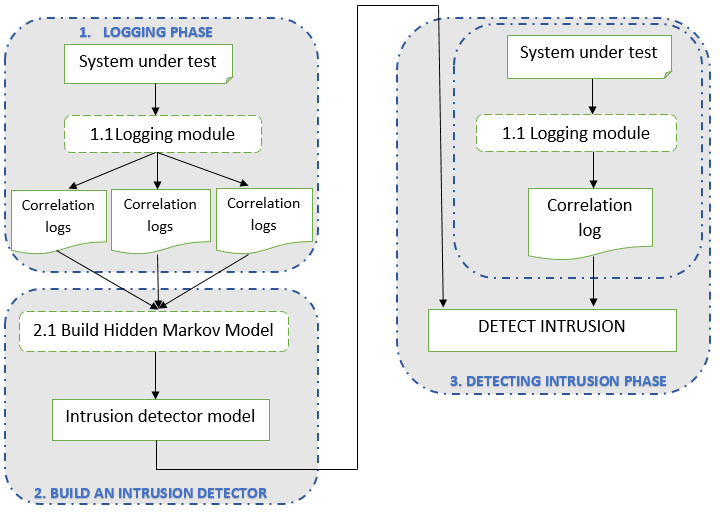
\includegraphics[scale=0.65,keepaspectratio = true]{Graphics/CORGIDSWorkflowNew.png}
    \caption{Workflow of CORGIDS}
    \label{fig:workflow}
\end{figure}

\ac{CORGIDS} workflow can be broken down into three main phases, namely, a) Logging Phase; b) Building an Intrusion Detector Phase; and c) Detecting Intrusion Phase. Each of the phases are explained below.

\begin{enumerate}
\item {Logging Phase}: The \textit{1. Logging Phase} in ~\autoref{fig:workflow} is the starting point for building an intrusion detector and for deploying it on a system for which intrusion detection is desired. \ac{SUT} is an input to this phase and is passed through the \textit{1.1 Logging module} in which it is manually instrumented to collect the values of the correlated properties\footnote{The approach of manually instrumenting the code to collect logs has been used by prior work~\cite{chen2018learning,aliabadi2017artinali}}. These properties are chosen by the user of the intrusion detection system based on the general knowledge of the \ac{SUT}. This phase will ensure that the traces which contain the values of the properties while the system is running are collected. Also, it is assumed that the source code of the \ac{SUT} is available and can be modified for instrumentation - this is reasonable as the developer of the system will deploy \ac{CORGIDS}. At the end of this \textit{logging phase}, the system traces containing the values of the logical properties of the \ac{SUT} are collected.

\item {Building an Intrusion Detector Phase}: In this phase, the system traces collected from the \textit{Logging Phase} are used to build an \ac{HMM} which behaviorally represents the \ac{SUT}. The pseudo code of the algorithm for building an intrusion detector is described below. To build an intrusion detector the system traces are fed into the \ac{HMM} model for its training in Line 1 in \textit{Procedure buildAnIntrusionDetector}.

\begin{algorithm}
  \caption{Building an intrusion detector}
  \textbf{Procedure buildAnIntrusionDetector (\textit{logs})}\;
  \nl \textit{trainedModel} = trainHMMModel (\textit{logs})\;
  \nl \ForEach{$l \in \textit{logs}$}{
    \textit{logLikelihood(i)} = log(\textit{trainedModel(l)})\;
    \textit{S} = sum of all \textit{logLikelihood(i)'s}\;
    }
  \nl \textit{M} = mean of \textit{S}\;
  \nl return \textit{trainedModel}, \textit{M}\;

  \textbf{Procedure trainHMMModel (\textit{logs})}\;
  \nl \ForEach{$\textit{hiddenStates} \in \{2, 3, \dots, J\}$}{
    \textbf{create an HMM model} \textit{model}(i)\;
    \textit{logLikelihood(i)} = log(\textit{model}(i))\;
    \nl \textbf{if} (\textit{logLikelihood}) \textless \textit{threshold} \textbf{then}\;
    \nl return \textit{model}(i)\;
  }
\end{algorithm}


Training of an \ac{HMM} is begun in \textit{procedure trainHMMModel} in Line 5, by varying the number of \textit{hiddenStates}. The number of hidden states is a free parameter of an \ac{HMM} which needs tuning in order to create a model which can be used for intrusion detection. Iteration begins with \ac{HMM} \textit{model(i)} with the starting value of two hidden states and is kept on increasing by one (Line 5). The log likelihood of the \textit{model(i)} is calculated which represents the goodness of the \textit{model(i)} fit of the model to the data that was used for constructing it.
The log likelihood is stored in variable \textit{logLikelihood(i)} as shown in Line 5. The \textit{threshold} in Line 6 represents the minimum difference between the current and previous \ac{HMM} log likelihood. Using threshold as a stopping criteria for \ac{HMM} has also been used in prior work~\cite{ferrer2000influence}. The best \ac{HMM} is returned in Line 7 with its parameters as the model to be used for intrusion detection. At this point the \textit{trainedHMMModel} is used to calculate the log likelihood for each of the training system traces (Line 2). As a by product, the mean of log likelihood is calculated (Line 2) to get the estimated log likelihood value \textit{M} (Line 3) for a training log. \textit{M} is then used for comparison in the later steps to detect intrusion. Creating \ac{HMM} by increasing the number of hidden states uses a significant amount of memory and computational power.
However as this phase needs to be carried out just once for a \ac{SUT}, it is not a major bottleneck. Once the intrusion detector \ac{HMM} is created, it can be used to detect an anomaly in the next phase. 

\item {Detecting Intrusion Phase}: This phase starts with the \textit{Logging Phase} which is used to collect the system trace from the \ac{SUT} while it is running. In this phase, only the system trace corresponding to the running \ac{SUT} is collected, rather than many different system traces. 
The trace generated is then used together with the intrusion detector built in the \textit{Building an Intrusion Detector Phase}. Using the \ac{HMM} model and its saved parameters, the log likelihood of the current system trace is calculated and compared with the mean log likelihood \textit{M} calculated in the \textit{Building an Intrusion Detector} in Line 6. If the log likelihood of the system trace is less than a specified range ($\delta$) from \textit{M}, it signifies that the system trace does not follow the behavior which was observed when the \ac{HMM} was being trained. 
The specified range ($\delta$) is found by running a sensitivity analysis (Section \ref{sensitivityAnalysis}). Further, as the system traces used for building the \ac{HMM} were assumed to be correct (i.e., not attacked), this implies that the current system trace represents a system under attack.  
Thus, current state of the \ac{SUT} is flagged to be malicious. 
\end{enumerate}


\section{Example}

\begin{figure}[ht]
    \centering
    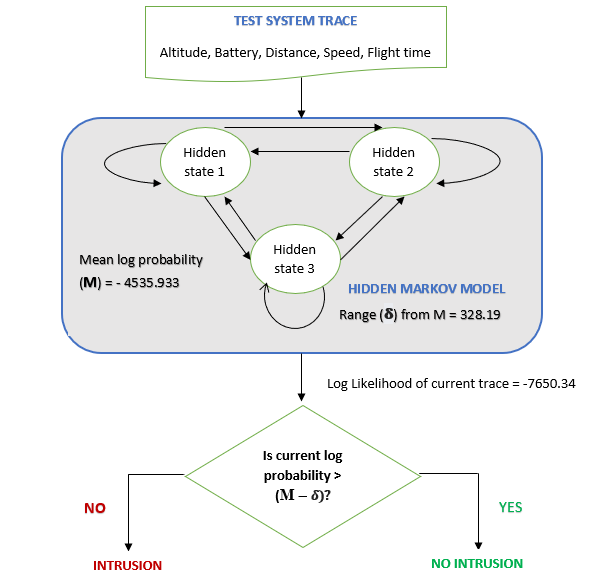
\includegraphics[scale=0.75,keepaspectratio = true]{Graphics/CORGIDSApproach.png}
    \caption{Approach of CORGIDS}
    \label{fig:approach}
\end{figure}

The earlier example of an \ac{UAV} from ~\autoref{ch:Introduction} is used in this section to illustrate how \ac{CORGIDS} can be used to detect intrusions in ~\autoref{fig:approach}. As described in chapter ~\autoref{ch:Introduction}, an \ac{UAV} has physical properties such as the current altitude, battery percentage left, distance traveled, current speed and flight time. These physical properties are correlated to each other as per the laws of physics. The approach which will be used to detect an intrusion in an \ac{UAV} is elaborated, using the work-flow described in ~\autoref{fig:approach}. Distance spoofing attack scenario of the \ac{UAV} is used as an example. This attack is explained in detail in ~\autoref{ch:Attacks}.

First the \textit{Logging Phase} starts, where the \ac{UAV} is instrumented to collect the correlated properties such as altitude, battery percentage left, distance traveled, speed and flight time. The above properties are collected at regular intervals of time to form the system traces. A section of the sample system trace collected is shown in Table~\ref{tab:nonFaultyCorrelationLog}. In the trace, it can be observed that all the properties are correlated  with each other, and that the correlations are fairly stable. For instance, if the \textit{Speed} of the \ac{UAV} increases, the \textit{Distance traveled} will also increase proportionally. Further, the \textit{Distance traveled} property can have values that are either increasing or stagnant. Multiple iterations of the \ac{UAV} were run by varying the routes it travels, to collect non-faulty system traces from it.

\begin{table}
\centering
  \caption{Slice of a non-faulty system trace obtained while flying an UAV on a random route}
  \label{tab:nonFaultyCorrelationLog}
  \scalebox{0.9}{
  \begin{tabular}{|p{1.2cm}|p{1.2cm}|p{1.85cm}|p{0.9cm}|p{1.7cm}|}
 \toprule
\textbf{Altitude (m)}&\textbf{Battery left (\%)}&\textbf{Distance traveled (m)}&\textbf{Speed (m/s)}&\textbf{Flight time (s)}\\
  \hline
..&..&..&..&..\\
40&89&42.1445&1&38.32\\
40&89&44.2563&2&39.342\\
40	&89	&47.2397	&3	&40.356\\
40	&89	&51.0202	&3	&41.376\\
40	&88	&55.2434	&4	&42.345\\
40	&88	&59.5897	&4	&43.346\\
40	&88	&64.1632	&4	&44.335\\
41	&88	&68.8979	&4	&45.323\\
41	&88	&73.7389	&4	&46.351\\
41	&87	&78.6564	&4	&47.448\\
41	&87	&83.6196	&4	&48.551\\
41	&87	&88.6138	&4	&49.61\\
41	&87	&93.627	    &5	&50.604\\
41	&86	&98.6659	&5	&51.507\\
..&..&..&..&..\\
\hline
\end{tabular}
}
\end{table}

\begin{table}
\centering
\caption{Slice of a faulty system trace obtained while an UAV was flying on a random route and infected by distance spoofing attack}
\label{tab:faultyCorrelationLog}
\scalebox{0.9}{
\begin{tabular}{|p{1.2cm}|p{1.2cm}|p{1.85cm}|p{0.9cm}|p{1.7cm}|}
\toprule   \textbf{Altitude (m)}&\textbf{Battery left (\%)}&\textbf{Distance traveled (m)}&\textbf{Speed (m/s)}&\textbf{Flight time (s)}\\
  \hline
..&..&..&..&..\\
 40 & 89 & 42.7868 & 1 & 38.206 \\
 40 & 89 & 45.2942 & 2 & 39.279\\
 41 & 89 & 48.6934 & 3 & 40.272\\
 42 & 89 & 42 &	4 &	41.261\\
42&	88&	57.0199&	4&	42.267\\
43&	88&	46&	4&	43.285\\
43&	88&	66.0254&	4&	44.357\\
44&	88&	70.7879&	4&	45.347\\
44&	87&	65&	4&	46.292\\
45&	87&	80.5709&	4&	47.37\\
46&	87&	85.5441&	4&	48.386\\
46&	87&	49&	4&	49.373\\
47&	86&	54&	4&	50.367\\
47&	86&	100.6006& 4&	51.402\\
..&..&..&..&..\\
\hline
\end{tabular}
}
\end{table}
In the second phase, \textit{Build an Intrusion Detector}, the system traces collected from \textit{Logging Phase} are used. \ac{HMM} are generated, \textit{model(i)}, by varying the number of hidden states in line 5 in the given algorithm. Then for each of the \textit{model(i)} generated, the \textit{logLikelihood(i)} is calculated in line 5 to determine if the \textit{model(i)} fits the data used for constructing it. To accomplish this, the difference in \textit{logLikelihood(i)} is compared to the \textit{threshold} in line 6 and if the \textit{threshold} is met, \textit{model(i)} is returned in line 7. It was found that an \ac{HMM} with 15 hidden states is the one which met the threshold. As showing 15 hidden states in the ~\autoref{fig:approach} will clutter it, we simplified the model by showing only 3 hidden states. Further, in lines 2 and 3, the sum of \textit{logLikelihood's} for all the correlated logs \textit{S} is calculated from which \textit{M} (mean log likelihood) = $-4535.933$ is extracted.

To demonstrate how an attack will be detected by \ac{CORGIDS}, we consider an attack where the attacker decides to spoof the values of distance traveled found inside the data packets being transferred from the \ac{UAV} to the \ac{GCS}. An \ac{UAV} periodically send the flight data to the \ac{GCS} to keep it updated about its whereabouts. To intervene the working of \ac{UAV}, the attacker gains access to the communication channel between the \ac{UAV} and \ac{GCS}. Now, an attacker can easily change the contents of the data packets being transferred.

In the final phase, when the \ac{UAV} is deployed in production, the \textit{Detecting Intrusion Phase} is active in the \ac{GCS} and uses the current system trace produced from the logging module along with the trained HMM to detect intrusion. A slice of the faulty-system trace is shown in Table~\ref{tab:faultyCorrelationLog}. As can be observed, the values of distance traveled are changing but do not follow the correlations observed in the earlier trace in Table~\ref{tab:nonFaultyCorrelationLog}. As only the distance traveled values have been tampered with, leaving other logical properties intact, we get a correlation which is different from the one that is expected by the trained \ac{HMM}. This results in the difference between the mean and current log likelihood values being greater than the threshold value - say ($\delta$). From ~\autoref{fig:approach}, the log likelihood of the current system trace is more than $\delta$ from the \textit{M} (mean log likelihood). Therefore, \ac{CORGIDS} flags the current state of the \ac{UAV} to be \textit{malicious}. The value of the threshold used in this example, ($\delta$) = $328.19$ is determined experimentally in section \ref{sensitivityAnalysis}. 


\endinput
=====================================================================

%% The following is a directive for TeXShop to indicate the main file
%%!TEX root = main.tex

% ===========================================================================================
\chapter{\textbf{Experimental Setup}}
\label{sec4:ExperimentalDetail}

This chapter first describes the details of the two test-beds on which CORGIDS was tested and the attacks to be planted. It then discusses the experimental procedures, and the experimental parameters that were chosen. Finally, it presents the evaluation criteria which will be used in ~\autoref{sec6:Evaluation}.

\section{Test-beds}
To demonstrate that CORGIDS is generic, two CPS test-beds were chosen on which the experiments were carried out. These test-beds contain correlated properties and a predefined framework according to which the properties change their values. 
\begin{enumerate}
\item Unmanned Aerial Vehicle (UAV): 


An UAV, commonly known as a drone, is a type of aircraft different from others mainly because it does not have a pilot aboard. UAV's periodically send the flight data to the GCS to keep it updated about its whereabouts.
 
A UAV mainly consists of sensors, control logic and actuators forming a closed loop. The sensors sense the current state of the UAV and its environment and pass it on to the controller, which makes the decision about the next step to be taken. The decision taken is then sent to the actuator - this loop runs infinitely while the UAV is in operation. ArduPilot's Software in the Loop (SITL) ~\cite{ArdupilotSITL} was used for the experiments. ArduPilot is an open-source autopilot software and is vastly deployed on various vehicle systems. SITL was chosen as the test-bed on a local machine due to lack of a real UAV.  


\begin{figure}%
    \centering
    \subfloat[Real drone]{{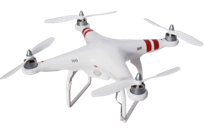
\includegraphics[width=6cm]{Graphics/drone.png} }}%
    \qquad
    \subfloat[ArduPilot's SITL]{{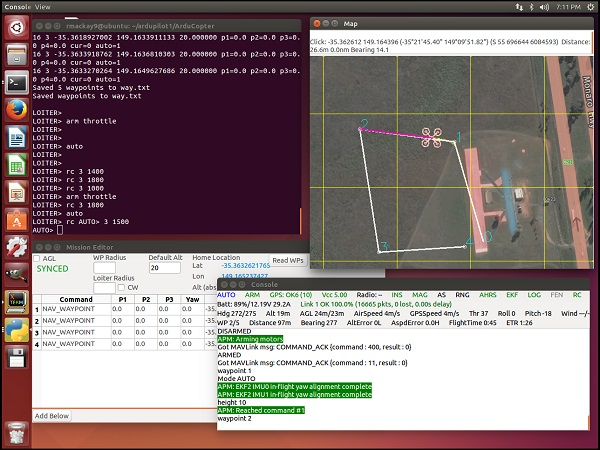
\includegraphics[width=6cm]{Graphics/sitl.jpg} }}%
    \caption{Drones}%
    \label{fig:drone}%
\end{figure}


\item Smart Artificial Pancreas (SAP): SAP is a device used by the diabetic patients to automatically analyze the insulin dosage to be injected into the patient based on the blood glucose level. SAP helps in reducing human error and analyzes the current blood glucose levels regularly at fixed intervals of time. A SAP consists mainly of i) a blood glucose monitor, which reads the blood glucose levels of the patients at regular interval of time, ii) a controller, which based on the blood glucose values decides the insulin that needs to be injected, iii) an insulin pump, which based on the value generated by the controller, injects a specific amount of insulin into the patient. Open Artificial Pancreas System (OpenAPS) an open source SAP was used to evaluate CORGIDS. OpenAPS implements the controller part of the SAP, and has been used in prior studies~\cite{aliabadi2017artinali}. As there was no real patient, I used the simulated values from blood glucose monitor and the insulin pump for our experiments. The values of blood glucose  were taken from the test cases provided by OpenAPS, instead from the blood glucose monitor. These values were then served as input to the OpenAPS to get the amount of insulin required by the patient. The OpenAPS controller was installed on a Raspberry Pi 3 microprocessor to evaluate the memory and performance overhead of CORGIDS.

\begin{figure}[ht]
    \centering
    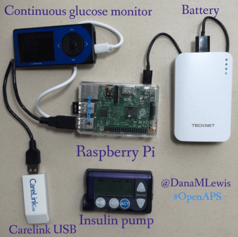
\includegraphics[scale=0.55,keepaspectratio = true]{Graphics/openaps.png}
    \caption{Components of an OpenAPS platform}
    \label{fig:OpenAPS}
\end{figure}
\end{enumerate}

\section{Experimental Procedure}
To evaluate CORGIDS's efficacy, the process of attack detection was partitioned  into two phases, namely training phase and testing phase. The system traces obtained from SUT were randomly divided into training and testing batches. The training phase is the one in which the intrusion detector is trained from the non-faulty system traces that are randomly assigned. Sensitivity analysis is also performed to analyze the value of the parameters which have the most impact on the performance of the intrusion detector. For instance, for the UAV testbed, routes which the UAV used as the flight plan were randomly generated. Therefore, after having the UAV simulator fly on all the randomly generated routes, the non-faulty system traces were obtained. These logs were then randomly distributed for training and testing phases. In the testing phase, the intrusion detector which was built in training phase, was used to find out if an intrusion was correctly detected. The results were then used to gauge the performance of CORGIDS based on the evaluation criteria. In order to reduce variability, five-fold cross validation was run for each of the attacks described above.

%CORGIDS is implemented in Python and spans over 200 lines of code.


\endinput
=====================================================================
% EOF
%% The following is a directive for TeXShop to indicate the main file
%%!TEX root = main.tex

% ===========================================================================================
\chapter{\textbf{Attacks description and detection}}
\label{ch:Attacks}

In this chapter, the attacks that were emulated on each test-bed are discussed. The attacks that are discussed here are  targeted attacks, which means that they specifically target physical properties of the two CPS platforms. Note, that the attacks designed for both the test-beds are intentionally stealthy, i.e. it is expected that the attacker wants to remain undetected while introducing some malicious content to accomplish its goal. Also, attack trees are used for designing attacks on the test-beds. These attack trees are based on prior attacks on very similar systems, thus making them realistic and appropriate for testing CORGIDS.


\section{Attacks on UAV}

\begin{figure}[ht]
    \centering
    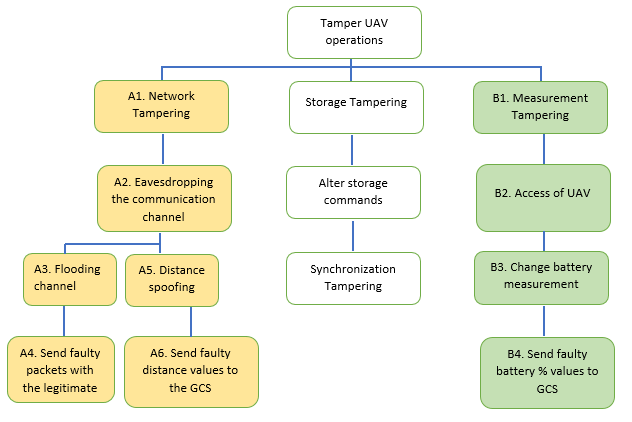
\includegraphics[scale=0.55,keepaspectratio = true]{Graphics/AttackTreeUAVNew.png}
    \caption{Attack tree for UAV}
    \label{fig:attackTreeUAV}
\end{figure}
As discussed above, an UAV regularly transmits flight data to the GCS, so that it can be tracked throughout its flight. The GCS based on the flight data received interprets if the UAV is following the instructed guidelines or has drifted from it. An attack tree for faulty UAV operations (shown in Figure~\ref{fig:attackTreeUAV}) was formulated, based on attacks introduced in previous work~\cite{javaid2012cyber, mitchell2012specification}. There are three branches in this tree, namely, i) Network Tampering; ii) Storage Tampering; and iii) Measurement Tampering. Two out of the three branches were used to develop attacks which are discussed below.

\begin{itemize}
\item {\bf Battery Tampering Attack (Block B1-B4)}: This attack occurs when an attacker is able to tamper with the control logic of the UAV by hacking it. By changing the control logic, the attacker can change the decisions that are made based on the input physical properties from the sensors. Obtaining the access of the UAV is not an unreasonable condition mainly due to the availability of tools capable of achieving the same ~\cite{pleban2014hacking, rodday2016exploring}.
In this attack, the attacker can change the part of the code where the percentage of battery left in the UAV is being sent to the GCS. The original value of percentage battery left in the UAV can be substituted with a value greater than the current value, to lead the GCS into the false understanding that the UAV has plenty of battery left in it. Specifically, if the attacker through eavesdropping the communication channel, knows that the battery decreases at a particular rate, it can then send faulty values to make the GCS believe that battery is depleting at a decreased rate to accomplish the motive. Eventually, reaching to a point where the UAV crashes on the ground due to battery drainage, and leads to the possession of sensitive data by the attacker. As I did not have access to a real UAV, the experiments on ArduPilot (a real time simulator for UAV) were performed on a local machine. Therefore, I had access to the UAV and modified its control logic to plant this attack in the code itself.

\item {\bf Flooding Attack (Block A1-A4)}: The flooding attack occurs when the communication channel between the UAV and GCS is compromised. In this scenario, an attacker can mount the attack by flooding the communication channel by the sending the extra packets along with the ones destined to be received by the GCS~\cite{pleban2014hacking}. The motive of this attack could be populating the channel so that the GCS is unable to infer the correct whereabouts of the UAV thereby, leading the attacker to control and use the UAV as desired. The extra packets being sent can  contain physical properties which are different from the legitimate ones. However, we assume that the attacker is stealthy and chooses values close to the real ones to avoid detection. 

To achieve this attack, faulty data packets were injected into the communication channel between UAV and GCS.

\item {\bf Distance Spoofing Attack (Block A (1,2,5,6))}: By sending a different value of the distance traveled instead of the original value, an attacker can falsely portray the current route or the current position of the UAV to the GCS. This attack can take place when an attacker eavesdrops on the communication channel to know the format of data being transmitted. This knowledge then can be used to spoof the value of the distance covered in the data packets being sent to the GCS. The motivation behind this attack can be that the attacker wants to fool the GCS by leading it to believe that the UAV is following a different schedule/route than the planned one. This attack is mounted by spoofing false distance traveled data into the communication channel between the GCS and UAV. Similar to flooding attack, the communication channel was intercepted to send spoofed values for the distance traveled property to the GCS.
\end{itemize}


\section{Detection of attacks on UAV}
\begin{itemize}
\item {\bf Battery Tampering Attack}: As detailed in the attack description, the attacker changes only the battery values in a data packet which also contains other correlated properties such as distance traveled, altitude, speed, and flight time. When this data is received by the GCS with CORGIDS enabled on it, the trained HMM model in the intrusion detector module detects an abnormal activity. A malicious activity is detected because the correlation expected by the HMM is not the same as received by it, mainly due to the difference in the relationship of battery with the other properties in the data packet. As a result, the log likelihood of the current system trace comes out to be less than the intrusion detector, which makes it faulty. This leads to raising of an alarm by the GCS.

\item {\bf Flooding Attack}: To detect this attack, the data packets that are received by the GCS are fed into the intrusion detector module of CORGIDS. A key point to note here is that, if the UAV sends one data packet per second to the GCS, the data packets received at the GCS end, will be greater than the number of packets sent by the UAV, because of the flooding attack. The trained HMM model will detect a malicious activity as the number of data packets which are used for decision making are greater than the case when there is no flooding attack. This will lead to a lesser log likelihood of the current data packets than the trained HMM, thus flagging the current state as anomalous.

\item {\bf Distance Spoofing Attack}: When spoofed messages reach the GCS, they are given to the trained HMM model to find out discrepancy, if any. An important thing to note here is that the number of data packets sent by the UAV and received by the GCS are same. However, in some packets the distance traveled by UAV is spoofed to falsely portray that it is following a different route or may be the sensors are returning some faulty values. However, the correlation between the distance traveled and other flight data parameters from a mix of faulty and non-faulty packets, is not what is expected by the trained HMM. Thus, the intrusion detector flags the current state to be anomalous as the log likelihood of the data packets fed into it is lesser than expected.
\end{itemize}

\section{Attacks on SAP}
The correct execution of SAP is of vital importance as the life of the patient depends on it. As discussed above, SAP consists of three components: blood glucose monitor, controller and insulin pump forming a closed loop. The attacks that were derived for SAP are discussed below and take advantage of the communication channel and the access of the code for the controller \footnote{The attacks on SAP may seem similar to the ones proposed by~\cite{aliabadi2017artinali}, mainly because of similar attack names, but the attack and its detection methodology is totally different when compared to ours.}. An attack tree shown in Figure~\ref{fig:attackTreeOpenAPS} was built using the attacks demonstrated in prior work~\cite{aliabadi2017artinali, radcliffe2011hacking}. The attacks planted on SAP test-bed are based on the two scenarios described in it.
\begin{figure}[ht]
    \centering
    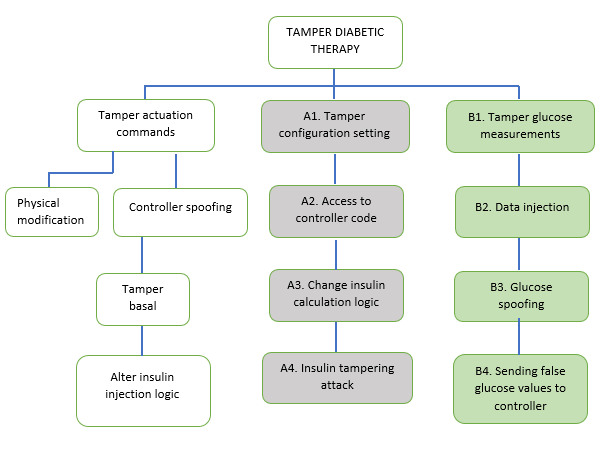
\includegraphics[scale=0.55,keepaspectratio = true]{Graphics/AttackTreeSAPNew.png}
    \caption{Attack tree for SAP}
    \label{fig:attackTreeOpenAPS}
\end{figure}

\begin{itemize}
\item {\bf Insulin Tampering Attack (Block A1-A4)}: Similar to battery tampering attack on an UAV, insulin tampering attack also occurs when the attacker hacks the controller unit of the system i.e., OpenAPS~\cite{radcliffe2011hacking}. After hacking, the attacker can modify the logic where the rate of insulin is calculated, based on the input blood glucose values sampled from the patient. This will lead to injection of faulty insulin dosage into the patients body which can prove fatal. I used the Raspberry Pi 3 for our SAP experiments and changed the control logic of the OpenAPS to reflect this attack. After the attack had been planted, the insulin dosage command sent out by the controller was faulty as expected.

\item {\bf Glucose Spoofing Attack (Block B1-B4)}: The glucose spoofing attack modifies the value of the blood glucose contained in the data packets being sent from the patient. The incorrect value which will be substituted can be either greater than, or less than the measured blood glucose value. This change in the real value will lead the controller to calculate an incorrect value of insulin (though the logic through which insulin dose calculated is untouched), which will have harmful effects on the patient. This attack was mounted by injecting false data into the communication channel between the blood glucose monitor and the controller.
\end{itemize}

\section{Detection of attacks on SAP}
\begin{itemize}
\item {\bf Insulin Tampering Attack}: As the attacker modifies only the insulin dosage while keeping the other properties the same, the intrusion detector is able to detect the attack, as the current correlation is not what it expects after its training phase. Similar to above attacks the log likelihood of the current system trace is less than that of the trained HMM, thus arousing suspicion.
\item {\bf Glucose Spoofing Attack}:  The intrusion detector module of CORGIDS receives the correlated properties which contains both faulty and non-faulty values of the blood glucose in it. Thus, based on this input data, the log likelihood generated by the current log differs from that expected by the trained HMM. This indicates that there is an intrusion in the current state of the SAP.
\end{itemize}

Although, the attacks that are demonstrated in this paper break the logical correlation directly, CORGIDS is also capable of detecting an anomaly which is generated through indirect attacks. For example, instead of changing the physical property like battery \% left in the battery tampering attack (this is a attack in which correlations are broken directly), we could change either the value of some variable (other than the physical variable) used in the UAV or alter other logic which does not directly effect the physical property. These changes will propagate in the program and ultimately reach the receiving end of the CPS (an actuator). If they do not, then the attack is likely to be harmless as the attacker cannot change the physical behavior of the CPS without modifying its outputs. 

\endinput
=====================================================================
% EOF
%% The following is a directive for TeXShop to indicate the main file
%%!TEX root = main.tex

% ===========================================================================================
\chapter{\textbf{Evaluation of \ac{CORGIDS}}}
\label{sec6:Evaluation}
In this chapter, the results from the sensitivity analysis and attacks seeded in ~\autoref{ch:Attacks} are presented. Also, additional experiments which provide more insight about how the tuning parameters of the trained HMM from phase two of workflow of \ac{CORGIDS} (\autoref{sec3:Approach}), effect the precision and recall were performed. The motive behind discussing the results achieved by \ac{CORGIDS} is to measure its performance in terms of the evaluation criteria described in this chapter.

\section{Sensitivity Analysis}
\label{sensitivityAnalysis}

Before evaluating \ac{CORGIDS}, a sensitivity analysis to find out the values of the three experimental parameters was performed. Sensitivity analysis is a study which determines how different values of an independent variable affect a particular dependent variable under a given set of assumptions. It can be used within given boundaries that depend on one or more input variables, such as the effect that changes in interest rates has on bond prices. The three experimental parameters for which the sensitivity analysis was carried out are as follows.

\begin{itemize}
\item Window size (\textit{w}): A window size is defined as the time duration which is under consideration for detecting an intrusion~\cite{zohrevand2016hidden} in a \ac{SUT}. A large \textit{w} means that greater historical data is given to the \ac{HMM} to decide of a malicious activity.
\item Acceptable range ($\delta$): An acceptable range defines a range within which the testing system trace's likelihood can vary from the mean log likelihood from the trained \ac{HMM}. A testing trace with the value within range from the specified mean will be marked to be similar to the training traces. If the value of $\delta$ is chosen to be large, it means that there is enforcement of loose control and allowing system traces with substantial variation from the trained \ac{HMM} to be considered benign.
\item Threshold of consecutive decisions ($\lambda$): Stateful tests~\cite{urbina2016limiting} are performed by maintaining the historical decisions of the \ac{IDS} and generating alert only if it goes above a chosen threshold. The intuition behind using the $\lambda$ is to look back at the historical decisions of the intrusion detector to see if there is really an anomaly or if it is just one time spike in the system. Greater value of $\lambda$ enforces more number of consecutive historical intrusion decisions to generate an alert.
\end{itemize}

The values of \textit{w}, $\delta$ and $\lambda$ were chosen based on the highest values of precision and recall (\autoref{sec:metrics}) achieved in this experiment. The results from sensitivity analysis are shown in ~\autoref{fig:sensitivityAnalysis}, ~\autoref{fig:sensitivityAnalysis_2} and ~\autoref{fig:sensitivityAnalysis_3}. \textit{w} is measured in minutes while $\delta$ in standard deviations. A key point to note here is that more the value of precision and recall for a set of experimental parameters, higher is the rate of detection. This experiment was carried out by varying one parameter at a time and keeping others constant. For instance, graph \textit{a} in ~\autoref{fig:sensitivityAnalysis} denotes the scenario where the \textit{w} is varied from 2 to 4 minutes while keeping $\delta$ = 1 and $\lambda$ = 2. Following similar pattern from  graph \textit{a}, the constant parameters will be swept , that is, $\delta$ and $\lambda$ from their lowest to the highest values. This forms the graphs \textit{a} - \textit{d} in ~\autoref{fig:sensitivityAnalysis}. Therefore, similar to ~\autoref{fig:sensitivityAnalysis}, other experiments were conducted by varying $\delta$ in ~\autoref{fig:sensitivityAnalysis_2} and $\lambda$ in ~\autoref{fig:sensitivityAnalysis_3}. This sensitivity analysis represents the data collected from the distance spoofing attack on the \ac{UAV} testbed. 
%Though similar analysis was performed for the other attacks on the \ac{UAV} and \ac{SAP}, due to space limitations they are not included here. 

From the graphs, it can be seen that the precision and recall are increasing as the \textit{w} is increasing from 2 to 4 minutes, while they are decreasing when the $\delta$ and $\lambda$ are increasing from 1 to 3 standard deviations and 2 to 4 decisions respectively. From this trend it can be inferred that the precision and recall are largest when the \textit{w} is large with small $\lambda$ and $\delta$. Similar trend was observed for other attacks on the two test-beds. The reason for the trend that was observed is that a \ac{HMM} requires substantial historical data to determine if there is some anomaly in the system. With lesser history (smaller window size), it is unable to correctly infer the current state of the system. Therefore, when a greater \textit{w} of 4 minutes is provided, it is able to create a more realistic model of the system, as the \ac{HMM} is now more behaviorally knowledgeable about the system after having a large \textit{w} and can now make decisions with higher likelihood, thus giving the best results for the least value of $\delta$ and $\lambda$.


An important point to note here is that though \ac{CORGIDS} is able to detect attacks even with less favorable values of \textit{w}, $\lambda$ and $\delta$, it achieves less precision and recall in doing so. On the other hand, if the results obtained from sensitivity analysis are used, higher values of precision and recall can be achieved. Therefore, either the lesser favorable parameters can be chosen and results can be obtained quickly at the cost of accuracy, or with the most favorable parameters, fewer \ac{FN} can be obtained, while incurring some latency.


\begin{figure}%
    \centering
    \subfloat[$\delta$ = 1 and $\lambda$ = 2]{{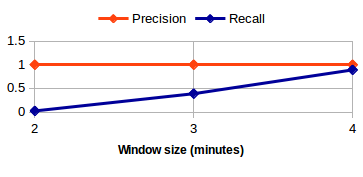
\includegraphics[width=0.50\textwidth]{Graphics/Spoofing_Window_1.png} }}%
    \subfloat[$\delta$ = 3 and $\lambda$ = 2]{{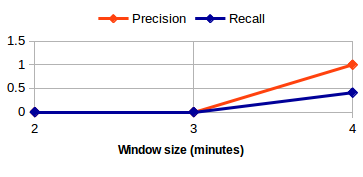
\includegraphics[width=0.50\textwidth]{Graphics/Spoofing_Window_2.png} }}%
    \qquad
    \subfloat[$\delta$ = 1 and $\lambda$ = 4]{{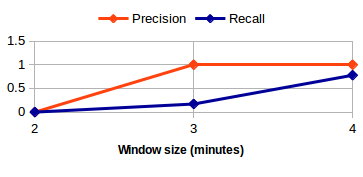
\includegraphics[width=0.50\textwidth]{Graphics/Spoofing_Window_3.png} }}%
    \subfloat[$\delta$ = 3 and $\lambda$ = 4]{{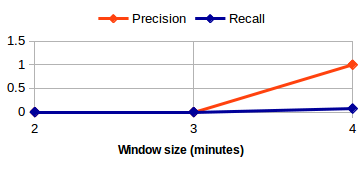
\includegraphics[width=0.50\textwidth]{Graphics/Spoofing_Window_4.png} }}%
    \caption{Sensitivity Analysis: Independent variables are $\delta$ and $\lambda$. Dependent variable is \textit{w}. The vertical axes in all figures are the values of precision and recall calculated after averaging 5 fold cross validation of test system traces.}%
    \label{fig:sensitivityAnalysis}%
\end{figure}

\begin{figure}
    \centering
    \subfloat[\textit{w} = 2 and $\lambda$ = 2]{{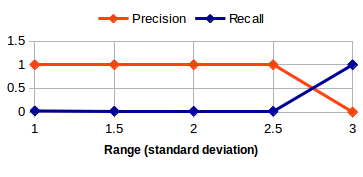
\includegraphics[width=0.50\textwidth]{Graphics/Spoofing_Range_1.png} }}%
    \subfloat[\textit{w} = 4 and $\lambda$ = 2]{{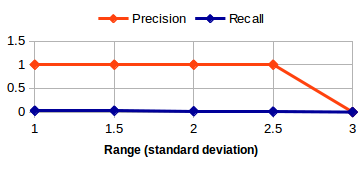
\includegraphics[width=0.50\textwidth]{Graphics/Spoofing_Range_2.png} }}%
    \qquad
    \subfloat[\textit{w} = 2 and $\lambda$ = 4]{{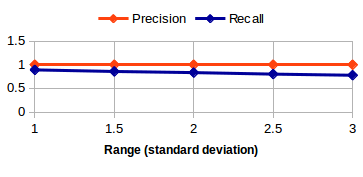
\includegraphics[width=0.50\textwidth]{Graphics/Spoofing_Range_3.png} }}%
    \subfloat[\textit{w} = 4 and $\lambda$ = 4]{{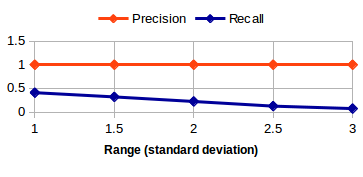
\includegraphics[width=0.50\textwidth]{Graphics/Spoofing_Range_4.png} }}%
    \caption{Sensitivity Analysis: Independent variables are \textit{w} and $\lambda$. Dependent variable is $\delta$. The vertical axes in all figures are the values of precision and recall calculated after averaging 5 fold cross validation of test system traces.}%
    \label{fig:sensitivityAnalysis_2}%
\end{figure}

\begin{figure}%
    \centering
    \subfloat[\textit{w} = 2 and $\delta$ = 1]{{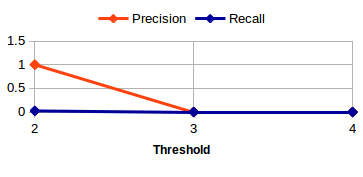
\includegraphics[width=0.50\textwidth]{Graphics/Spoofing_Decision_1.png} }}%
    \subfloat[\textit{w} = 2 and $\delta$ = 3]{{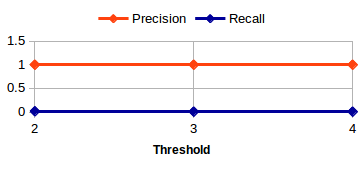
\includegraphics[width=0.50\textwidth]{Graphics/Spoofing_Decision_2.png} }}%
    \qquad
    \subfloat[\textit{w} = 4 and $\delta$ = 1]{{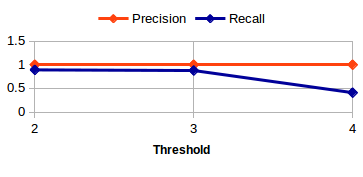
\includegraphics[width=0.50\textwidth]{Graphics/Spoofing_Decision_3.png} }}%
    \subfloat[\textit{w} = 4 and $\delta$ = 3]{{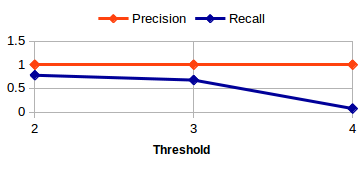
\includegraphics[width=0.50\textwidth]{Graphics/Spoofing_Decision_4.png} }}%
    \caption{Sensitivity Analysis: Independent variables are \textit{w} and $\delta$. Dependent variable is $\lambda$. The vertical axes in all figures are the values of precision and recall calculated after averaging 5 fold cross validation of test system traces.}%
    \label{fig:sensitivityAnalysis_3}%
\end{figure}

\section{Evaluation Criteria}
\label{sec:metrics}

Precision, recall, \ac{FP}, \ac{FN}, performance overheads and memory overheads were used to evaluate \ac{CORGIDS}. These metrics are explained below:

\begin{itemize}
\item Precision: For a malicious execution of \ac{SUT}, when an intrusion detector correctly detects an intrusion, is called precision. For an intrusion detector, the higher precision the better.
\item Recall: On the other hand, recall is the percentage when the \ac{SUT} execution was malicious and the intrusion detector correctly identified it among all the malicious \ac{SUT} executions. For an intrusion detector, the higher recall the better.
\item \acf{FP}: Represents the ratio of execution traces that were falsely reported as malicious to the total number of normal traces for a given \ac{CPS}.
\item \acf{FN}: Represents the ratio of malicious attacks that went undetected/unnoticed by the IDS to the total number of attacks for a given \ac{CPS}.
\item Performance Overhead: Performance overhead reflects the additional time taken, when \ac{CORGIDS} is deployed on the \ac{SUT}. It helps to determine if the time taken by the \ac{IDS} to detect intrusion is greater than the time taken to complete a closed loop once, in which case it is not very helpful to use an \ac{IDS}.
\item Memory Overhead: As the devices in which \ac{CORGIDS} will be used will be memory constrained, it is essential to calculate its memory overhead. Memory occupied by \ac{CORGIDS} on \ac{SUT} will be used to determine this overhead.
\end{itemize}

%As there wasn't a real \ac{UAV} and a simulator was used for the \ac{UAV} experiments, and therefore memory and performance overheads for \ac{UAV} test-bed were not calculated.

\begin{table}
\centering
  \caption{False Positive and False Negative obtained for CORGIDS on the two test-beds}
  \label{tab:results}
  \scalebox{0.9}{
  \begin{tabular}{|c|c|c|l|}
    \toprule
    \textbf{Testbed}&\textbf{Targeted Attack}&\textbf{FP (\%)}&\textbf{FN(\%)}\\
    \midrule
    \multirow{3}{*}{UAV}& Battery Tampering&0.0&12.20\\
                        & Flooding&0.0&11.30\\
                        & Distance Spoofing&0.0&12.80\\
    \hline
    \multirow{2}{*}{SAP}& Insulin Tampering&5.60&4.20\\
                            & Glucose Spoofing&2.80&8.40\\
    \hline
\end{tabular}
}
\end{table}


\begin{table}
\centering
  \caption{Comparison of Precision and Recall for OpenAPS platform}
  \label{tab:comparisonOfResults}
  \scalebox{0.9}{
  \begin{tabular}{|p{2.2cm}|p{2.0cm}|p{1.0cm}|p{1.0cm}|p{2.0cm}|p{1.8cm}|}
    \toprule
    \textbf{Methodology}&\textbf{Testbed}&\textbf{FP(\%)}&\textbf{FN(\%)}&\textbf{Precision(\%)}&\textbf{Recall(\%)}\\
    \midrule
    \multirow{2}{*}{ARTINALI}& SEGMeter&12&2.3&89.06&97.7\\
                        & OpenAPS&13.5&2&87.89&98\\

    \hline
    Zohrevand&Water&&& &\\
    et al.~\cite{zohrevand2016hidden}&Treatment&- &- & 78.87&81.4\\
     & System& & & & \\
    \hline
    Chen &Water &&&&\\
    et al.~\cite{chen2018learning}&Purification &- &15 &- &- \\
     &Plant& & & & \\
    \hline
    \multirow{2}{*}{CORGIDS}& UAV&0.00&12.10&100&87.90\\
                            & SAP&4.20&6.30&95.70&93.70\\

    \hline
\end{tabular}
}
\end{table}

For evaluating \ac{CORGIDS}, the value obtained for each of the three variables (\textit{w}, $\lambda$ and $\delta$) from the sensitivity analysis was used. ~\autoref{tab:results} contains the results for \ac{FP} and \ac{FN} for the two test-beds, namely, an \ac{UAV} and \ac{SAP} on which \ac{CORGIDS} was deployed. ~\autoref{tab:comparisonOfResults} compares our results to only those related papers~\cite{chen2018learning,zohrevand2016hidden,aliabadi2017artinali} which dynamically generate physical invariants \footnote{Note: For the research papers that were used for comparison with \ac{CORGIDS} for the \ac{UAV} and \ac{SAP} test-bed, the \ac{FP}, \ac{FN}, precision and recall values were directly used. Manual calculation of precision and recall for~\cite{aliabadi2017artinali} was made from the \ac{FP} and \ac{FN} values provided in their paper.}. We acknowledge that ~\autoref{tab:comparisonOfResults} does not provide a complete comparison as the test-beds, attacks and training and testing scenarios were different for each \ac{IDS}, however we include it here to provide better context about \ac{CORGIDS} performance. Later in ~\autoref{ch:comparisonwithrelatedwork}, a comprehensive comparison of CORGIDS with its related work is described.

Krotofil et. al. and Iturbe et. al.~\cite{krotofil2015process,iturbe2017feasibility} do not measure the performance of their methodology, and hence they could not be compared with \ac{CORGIDS}. In addition, precision and recall for \ac{CORGIDS} and the papers mentioned in ~\autoref{tab:comparisonOfResults} were calculated. To calculate the \ac{FP} and \ac{FN} values for \ac{CORGIDS} which will be used to generate precision and recall, \ac{FP} and \ac{FN} values from ~\autoref{tab:results} were averaged. However, comparison of the precision value of \ac{CORGIDS} with Chen et. al.~\cite{chen2018learning} could not be made, as the later did not provide it in their paper.  

\section{Experiment results} 
Based on the above described metrics, we now discuss the results of the experiments performed.

\subsection{Precision}
In this subsection, the precision achieved by seeding the attacks on the \ac{SUT} and using \ac{CORGIDS} to detect an intrusion is discussed. Also,  the precision achieved with prior work in  ~\autoref{tab:comparisonOfResults} is shown. As can be observed, \ac{CORGIDS} achieves a precision of 100\% and 95.70\% for the \ac{UAV} and \ac{SAP} platform respectively. In comparison, no other intrusion detector has a precision greater than 90\%. Specifically, \ac{CORGIDS} provides an 21.33\% improvement in precision over Zohravend et al. \cite{zohrevand2016hidden} and approximately 8.88\% over Aliabadi et al. \cite{aliabadi2017artinali} for the \ac{SAP} platform.

The reason behind the higher precision percentage for \ac{CORGIDS} is the use of correlations exhibited by the two CPS. \ac{CORGIDS} detects attacks by using an \ac{HMM} to infer if the current system trace exhibits the same trend with which it was trained. This is the reason that especially for the \ac{UAV} platform, the \ac{HMM} recognizes an anomaly with almost 100\% precision. The reason for comparatively low precision value for \ac{SAP} platform is the lack of traces. As the total number of traces for the \ac{SAP} platform were less, it led to even lower training traces, which eventually effected the modeling of the \ac{HMM}. For the experiments on both the test-beds, 70\%:30\% ratio for training and testing traces was maintained. However, the lack of availability of patient's diabetic therapy data led to a lower number of training traces. This, in turn negatively affected the training of the \ac{HMM} used by \ac{CORGIDS} for the \ac{SAP} platform.

\subsection{Recall}
The recall factor of \ac{CORGIDS} is discussed here and compared to the related work mentioned in ~\autoref{tab:results} and ~\autoref{tab:comparisonOfResults} respectively. From  ~\autoref{tab:comparisonOfResults}, it can be observed that \ac{CORGIDS} receives a high recall percentage among all the related work. Although, \ac{CORGIDS} does not have the highest recall, it is quite close to ARTINALI with 93.70\% for the \ac{SAP} platform. \ac{CORGIDS} improves the recall by 15.11\% when compared to  Zohravend et al.~\cite{zohrevand2016hidden}. On the other hand, \ac{CORGIDS} achieves 11.14\% lower recall than ARTINALI when both of them are compared with their lowest recall factors. 

 
\ac{CORGIDS} achieves lesser recall than ARTINALI~\cite{aliabadi2017artinali} mainly because the behavior of the \ac{SUT} under attack was stealthy and did not deviate much from the normal trend. As the deviation was less, the logical correlation between the properties seemed very similar to the one expected, thus the \ac{HMM} did not mark the state as anomalous, leading to some false-negatives. Chen et al. ~\cite{chen2018learning} do not provide recall factor, but give the value of \ac{FN} for their approach, the \ac{FN} value is compared to \ac{CORGIDS}, which is 15\%. This is higher than \ac{CORGIDS} \ac{FN} values of 12.10\% and 6.30\% for the two platforms. Chen et al. use \ac{SVM} for intrusion detection, while \ac{CORGIDS} uses \ac{HMM}. \ac{HMM} are able to better capture the sequence of states and their transitions in a \ac{CPS}, and hence \ac{CORGIDS} achieves lower \ac{FN} values.

\subsection{Memory overhead}
Measurements of the memory overhead of \ac{CORGIDS} running on the \ac{SAP} platform were also collected. The experiments were performed on a Raspberry Pi 3 with approximately 1 GB of RAM. We found that \ac{CORGIDS} consumes 36.15 MB when detecting intrusion. The reason behind this memory overhead is that \ac{CORGIDS} uses \ac{HMM} for intrusion detection. The trained \ac{HMM} model when loaded into memory along with the libraries required for it to generate a decision, requires more space. However, as \ac{CORGIDS} is used by controller to detect intrusion in the \ac{SUT}, and the controllers are not memory constrained as compared to the \ac{SUT}. For instance, in Raspberry Pi 3, it took only a fraction (36.15 MB) of memory from the 1 GB available RAM. Thus, we surmise that the memory overhead incurred by \ac{CORGIDS} is acceptable.

\subsection{Performance overhead}
Like memory overhead, performance overhead measurements were also taken from the Raspberry Pi 3 platform. The average of 10 executions was considered for the overhead tests.  
Ideally, the time taken to deduce a decision should be less that the execution cycle of the \ac{SUT}, in order for the intrusion detector to keep up with the system. The execution cycle time is the time taken to go though once the closed loop of a \ac{CPS}. The execution cycle time is important because it gives an idea of how much time the system takes to complete one loop of input from blood glucose sensors, to calculating the insulin dosage and sending the same to the insulin pump. It takes approximately 1.25 seconds for \ac{CORGIDS} to generate a decision based on the input correlated logs. This is negligible compared to the time taken by a single execution cycle of \ac{SAP}, which is about 5 minutes.

\bigskip
\textbf{Scalability of CORGIDS:} To understand the scalability of the overheads with \ac{HMM} size, the \ac{HMM} used for intrusion detection were varied. Thus, multiple \ac{HMM} were created by varying the tuning parameter, the number of \textit{hiddenStates}. The number of \textit{hiddenStates} were varied among {2, 5, 10, 15, 20}. We observed that the memory and performance overhead of \ac{CORGIDS} remains the same regardless of the number of \textit{hiddenStates} in the \ac{HMM}. This is could be because the libraries which are loaded along with the \ac{HMM} is the dominant factor in the time, and this does not depend on the number of \textit{hiddenStates} in the \ac{HMM}.

\section{Additional experiments}
We carried out additional experiments to gather more insight about how the \textit{precision} and \textit{recall} vary based on the type of trained \ac{HMM}.
We conduct experiments which include the variation of the two parameters which determine the type of trained \ac{HMM} that will be generated.
\begin{itemize}
\item Training threshold - Training threshold is used as a stopping criteria for training the \ac{HMM} in \textit{Building an Intrusion Detector} phase. This value signifies the maximum difference between current and previous \ac{HMM} log likelihood, if the current \ac{HMM} is the trained \ac{HMM}. We used the value of 0.5\% as the \textit{training threshold} in ~\autoref{sec3:Approach} based on the prior work~\cite{ferrer2000influence}. However, through this experiment we want to determine the effect that the change of this value has on intrusion detection capability of the trained \ac{HMM}. We sweep the value of training threshold from the values (0.35\%, 1\% and 2\%) with 0.5\% value already being used in our experiments.

\item Number of training traces - The number of training traces determine the context that the trained \ac{HMM} will have. Higher the number of training traces, more likely is that the \ac{HMM} will be equipped with different types of behavior exhibited by the \ac{CPS}. For our experiments, we kept the value of training to testing traces to be 70\% : 30\%. However, for this study we varied this ratio to see what effect it had on the precision and recall of the \ac{IDS}. Therefore, the ratio of training traces to testing traces was varied between (50\% : 50\%, 60\% : 40\% and 80\% : 20\%) with 70\% : 30\% ratio already covered in the above experiments.
\end{itemize}

Both parameters - training threshold and number of training traces - discussed above are varied one by one, i.e. while one is varied other is kept constant, and vice-versa. Also, this study was conducted for both the platforms - \ac{UAV} and \ac{SAP}.

\subsection{Additional results for UAV platform}
We conducted two experiments, one for each of the two parameters and summarize the results below.

\begin{itemize}

\item \textit{Training threshold}: By varying the training threshold and keeping the number of training to testing traces constant to 70\% : 30\%, we got the result shown in ~\autoref{fig:UAV_threshold}. Similar trend of precision and recall was observed for each of the individual value of training threshold as when the training threshold was 0.5\%. Also, it was seen that the training threshold did effect the recall factor of \ac{CORGIDS}. It can be seen that the recall increases as the training threshold decrease. So, for 0.35\% as the training threshold we get the maximum value of recall. However, the recall offered by training threshold value of 0.5\% is very close to the maximum recall value achieved in this experiments. Therefore, while using 0.5\% for the attacks which we reported in ~\autoref{ch:Attacks}, we did not sacrifice the intrusion detection capabilities of \ac{CORGIDS} by using an under-trained \ac{HMM}. On the other hand, it can also be seen that the precision remains unaffected by the change in training threshold, this could be because the trained \ac{HMM} which we got from each of the individual experiments was well trained about the benign behavior of the \ac{SUT}.

Another observation we made was that the time taken to get the trained \ac{HMM} model increased as the training threshold decreased. It was because, the maximum difference between the log likelihood's of the two \ac{HMM} was shrinking which led to creation of more \ac{HMM} until the threshold was met. However, as this training process needs to be done only once and that too on a non-constrained device, thus making the time consumed aspect not a road blocker.

\begin{comment}
\begin{table}
\centering
  \caption{Result by varying the \textit{training threshold} for the UAV platform}
  \label{tab:UAV_threshold_results}
  \scalebox{0.9}{
  \begin{tabular}{|c|c|c|}
    \toprule
    \textbf{Training threshold}&\textbf{Precision}&\textbf{Recall}\\
    \hline
    0.35\%& 100.0&90.70\\
    \hline
    0.5\%& 100.0 &89.20\\
    \hline
    1.0\%& 100.0&78.0\\
    \hline
    2.0\%& 100.0 & 74.50\\
    \hline
\end{tabular}
}
\end{table}
\end{comment}

\begin{figure}[ht]
    \centering
    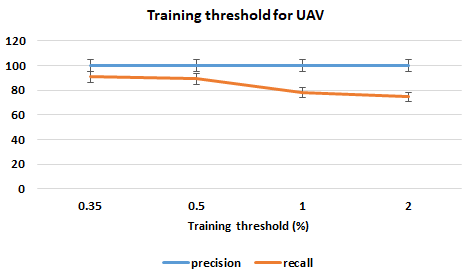
\includegraphics[scale=0.75,keepaspectratio = true]{Graphics/UAV_threshold.png}
    \caption{Result by varying the \textit{training threshold} for the UAV platform}
    \label{fig:UAV_threshold}
\end{figure}

\item \textit{Number of training traces}: By varying the training to testing traces ratio and keeping the training threshold at 0.5\%, we got the results described in ~\autoref{fig:UAV_traces}.
As can be observed, the number of training traces do affect the performance of \ac{CORGIDS}. Specifically, \ac{CORGIDS} achieve the best precision and recall when the training traces are maximum or near to the maximum value. Using 80\% or 70\% of the traces as training helped to achieve the recall of approximately 89 as opposed by lesser number of traces.

We see a dip in recall when the number of training traces decrease, because with fewer training data points, the \ac{HMM} does not get all the possibilities of the behavior that it can expect of the \ac{SUT}. Thus, more the number of training traces better the detection capability of \ac{CORGIDS}. Additionally, training the \ac{HMM} with different number of training traces did not make up a lot of time difference as compared to the experiment when the \textit{training threshold} was varied.

\begin{comment}
\begin{table}
\centering
  \caption{Result by varying the \textit{number of training traces} for the UAV platform}
  \label{tab:UAV_traces_results}
  \scalebox{0.9}{
  \begin{tabular}{|c|c|c|}
    \toprule
    \textbf{Number of training traces}&\textbf{Precision}&\textbf{Recall}\\
    \hline
    50\%: 50\% & 100.0 & 72.50\\
    \hline
    60\%: 40\% & 100.0 & 79.0\\
    \hline
    70\%: 30\% & 100.0 & 89.20\\
    \hline
    80\%: 20\% & 100.0 & 88.0\\
    \hline
\end{tabular}
}
\end{table}
\end{comment}

\begin{figure}[ht]
    \centering
    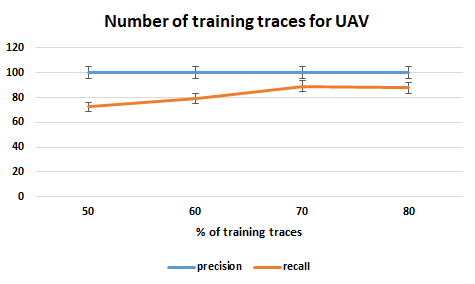
\includegraphics[scale=0.75,keepaspectratio = true]{Graphics/UAV_traces.png}
    \caption{Result by varying the \textit{number of training traces} for the UAV platform}
    \label{fig:UAV_traces}
\end{figure}

\end{itemize}

\subsection{Additional results for SAP platform}
We performed similar experiments for the training threshold and the number of training traces variables for the \ac{SAP} platform, with the results summarized below.

\begin{itemize}
\item \textit{Training threshold}: For this experiment, we used the same values of the training threshold from the above experiment involving the \ac{UAV} platform. That is, we varied the threshold between (0.35\%, 1.0\% and 2\%) with the experiments already conducted for the 0.5\% value in the attacks discussed in the ~\autoref{ch:Attacks}. The results are summarized in ~\autoref{fig:SAP_threshold}.

We see that the variation in the training threshold value has an effect on the recall of \ac{CORGIDS}. Particularly higher the value of training threshold, lower the recall of \ac{CORGIDS}, which means it is not able to detect malicious activities that well. However, the precision for all the experiments led to approximately similar value of 95. This could be because the HMM was able to capture the benign behavior of the \ac{SUT} with more precision. Further more, as the number of training traces for the \ac{SAP} platform were approximately 4 times less than the \ac{UAV} platform, it led to a very small number of training traces for each of the experiment conducted. Which is why the results of \ac{SAP} platform if compared with \ac{UAV} are lagging behind.

\begin{comment}
\begin{table}
\centering
  \caption{Result by varying the \textit{training threshold} for the SAP platform}
  \label{tab:SAP_threshold_results}
  \scalebox{0.9}{
  \begin{tabular}{|c|c|c|}
    \toprule
    \textbf{Training threshold}&\textbf{Precision}&\textbf{Recall}\\
    \hline
    0.35\% & 95.40 & 89.70\\
    \hline
    0.5\% & 95.70 & 93.70\\
    \hline
    1.0\% & 94.75 & 75.0\\
    \hline
    2.0\% & 95.30 & 57.50\\
    \hline
\end{tabular}
}
\end{table}
\end{comment}

\begin{figure}[ht]
    \centering
    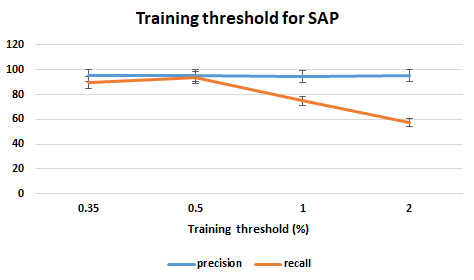
\includegraphics[scale=0.75,keepaspectratio = true]{Graphics/SAP_threshold.png}
    \caption{Result by varying the \textit{training threshold} for the SAP platform}
    \label{fig:SAP_threshold}
\end{figure}

\item \textit{Number of training traces}: By varying the ratio of training to testing traces and keeping the training threshold fixed at 0.5\%, we conducted experiments whose results are shown in~\autoref{fig:SAP_traces}. It is clearly seen that the number of training traces surely impacted the precision and recall of \ac{CORGIDS}. As anticipated, the few training traces led to less contextual behavior absorption for the \ac{HMM} which ultimately reflected on the evaluation metrics. For the attacks and result shared in ~\autoref{ch:Attacks}, we used 70\% : 30\% as the ratio and as can be seen from ~\autoref{fig:SAP_traces}, the precision and recall attained for these number of training traces achieve the maximum performance.

\begin{comment}
\begin{table}
\centering
  \caption{Result by varying the \textit{number of training traces} for the SAP platform}
  \label{tab:SAP_traces_results}
  \scalebox{0.9}{
  \begin{tabular}{|c|c|c|}
    \toprule
    \textbf{Number of training traces}&\textbf{Precision}&\textbf{Recall}\\
    \hline
    50\%: 50\% & 67.50 & 62.50\\
    \hline
    60\%: 40\% & 72.35 & 72.60\\
    \hline
    70\%: 30\% & 95.70 & 93.70\\
    \hline
    80\%: 20\% & 96.0 & 92.60\\
    \hline
\end{tabular}
}
\end{table}
\end{comment}

\begin{figure}[ht]
    \centering
    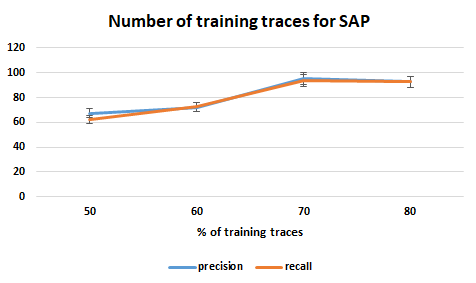
\includegraphics[scale=0.75,keepaspectratio = true]{Graphics/SAP_traces.png}
    \caption{Result by varying the \textit{number of training traces} for the SAP platform}
    \label{fig:SAP_traces}
\end{figure}

\end{itemize}

\section{Summary}

This chapter contains the results of sensitivity analysis which was performed to find out the values of three experimental factors which effected how the \ac{IDS} performed while detecting intrusion. It was found that as the window size increased and the acceptable range and threshold of consecutive decisions decreased, \ac{CORGIDS} performance was increasing, that is, fewer \ac{FP} and \ac{FN}. This observation was because the intrusion detector model uses \ac{HMM} and \ac{HMM} requires a slice of the current system trace for generating a result. If the slice of the trace will be small, it will lead to a narrow window of observations for the \ac{HMM}, thus not giving it enough data to analyze the current situation. Secondly, in this chapter we presented the results of prototyping \ac{CORGIDS} and using it for intrusion detection for the attacks mentioned in previous chapter. We use the two test-beds, an \ac{UAV} and a \ac{SAP} to prove that \ac{CORGIDS} is a generic IDS for \ac{CPS}. From the results we see that \ac{CORGIDS} achieve higher precision and recall as compared to the prior work. However, for \ac{SAP} the recall is less than ARTINALI due to lack of the system traces from which the \ac{IDS} was trained. Memory and performance overheads were also measured for the \ac{SAP} test-bed which indicated that \ac{CORGIDS} required approximately 36 MB of memory and took 1.25 seconds to generate a result - benign or malicious.

\endinput
=====================================================================
% EOF
%% The following is a directive for TeXShop to indicate the main file
%%!TEX root = diss.tex

\chapter{Comparison with related work}
\label{ch:comparisonwithrelatedwork}

To provide an detailed comparison with the related work, we choose those \ac{IDS} which are similar to \ac{CORGIDS} from our related work. This makes ARTINALI the only \ac{IDS} which can be used for comparison purposes as it is generic and designed for \ac{CPS}. All the other \ac{IDS} discussed were built keeping in mind a particular \ac{CPS}, thus were incapable of being applied to any other test-beds. Therefore, in this chapter we discuss the comparison experiment that we performed, followed by its results.

\section{Experimental setup}
In this chapter, we discuss how we carry out the comparison with ARTINALI which includes the test-beds, attacks carried out, collection of system traces and determining invariants. 
\begin{itemize}
\item Test-beds - We chose to use two test-beds - \ac{UAV} and \ac{SAP} - used in this study as the base for the comparison. These test-beds are valid for comparison because \ac{CORGIDS} already demonstrated its efficacy on these platforms. \ac{SAP} was also used by ARTINALI.

\item Attacks - To provide an even playing ground and completeness, we conducted this experiment by taking into account all the attacks that were used in both the \ac{IDS} - ARTINALI and \ac{CORGIDS}. Particularly, we consolidate targeted and arbitrary attacks from ARTINALI and targeted attacks from \ac{CORGIDS} to form a super set which was eventually used for evaluation. For example, for the case of \ac{SAP} platform which was common for both the \ac{IDS}, we combined the targeted attacks from both \ac{IDS} - ARTINALI and \ac{CORGIDS} - which were used to measure the detection capabilities. However, as \ac{CORGIDS} did not use arbitrary attacks as mentioned in ~\autoref{ch:Attacks}, all the arbitrary attacks from ARTINALI were used as a measure for both the \ac{IDS}.
Arbitrary attacks or fault injections represent the building blocks of the attacks that can occur as zero day attacks, as opposed to the targeted attacks which are designed to exploit a particular feature of the system under attack. The arbitrary attacks used by ARTINALI are:

\begin{itemize}
\item Data mutation, these attacks alter the run-time values of data variables in the code of the \ac{CPS}.
\item Branch flipping attacks randomly flip branch conditions to lead to an abnormal execution flow in the \ac{CPS}.
\item Artificial delay insertion adds some delay in normal execution of the program in \ac{CPS}.
\end{itemize}

As a result of the above mentioned arbitrary attacks, following observations were made in the \ac{CPS}, i) \textit{Crash}, by the introduction of the attack, the system resulted in a crash, ii) \textit{Hang}, means that after the introduction of the attack the system failed to do anything (was unable to perform any operation), iii) \textit{\ac{SDC}}, during the attack the operation of the system deviated from its non-malicious outcome, however, the system continued to function, and iv) \textit{No Corruption}, no visible changes were observed during run-time, which could differentiate it from the non-malicious system behavior. Only \ac{SDC} and no corruption attacks are taken into account while judging the performance of both the \ac{IDS}, as they are difficult to detect and need an \ac{IDS}. This is because, the other two system behaviors (crash and hang) are easily detected and they do not necessarily need an \ac{IDS} to observe that something is wrong with the system. 

For this comparison, we manually seed each of these faults in the source code of the respective test-beds, by randomly sampling the corresponding program points in the program’s code of the \ac{CPS}. We manually chose the fault injection points randomly before performing the experiment.

\item Collection of system traces - To avoid any bias in the traces which were used for building the \ac{IDS} and consecutively for checking intrusion, we used the same flight plans for \ac{UAV} platform, and the same glucose readings for the \ac{SAP} platform, for both \ac{IDS}. These traces were then randomly divided into 70:30 ratio for training and testing purposes for each \ac{IDS}.

\item Choosing invariants for modeling \ac{IDS} - As \ac{CORGIDS} had previously used the two test-beds for intrusion detection, we already had the physical variables to be used for modeling/deducing the \ac{CPS} behavior. ARTINALI, on the other hand, had data, event and time invariants for only the \ac{SAP} platform, therefore, we had to extract those invariants for the \ac{UAV} platform. ARTINALI defines an event as ``an instance of an action that leads to a change of condition., e.g. message send/receive, sensor data reading or activating insulin injection". Based on this definition and also the \ac{CPS} traces they collected for smart meter and \ac{SAP} test-beds, we chose the invariants for \ac{UAV} platform. 31 system calls were found which were marked as events, and for those events(i.e., function calls), the data variables that were present inside became the data invariants. For instance, functions which read the sensor data in the \ac{UAV} (latitude, longitude, speed, etc.) were chosen as events. Following this, the Data-Event-Time interplay was calculated by ARTINALI's code\cite{ARTINALI}, after we provide the \ac{CPS} traces required.
\end{itemize}

\section{Comparison on \ac{UAV} Platform}
This chapter consists of the attacks - targeted and arbitrary - which were used to determine the efficiency of both ARTINALI and \ac{CORGIDS} for the \ac{UAV} platform. We discuss the targeted and arbitrary attacks one by one.


\subsection{Targeted attacks}
The attacks - battery tampering, flooding and distance spoofing - described in this chapter are targeted attacks from \ac{CORGIDS}, as ARTINALI did not have any experiments on the \ac{UAV} platform.
The results of these attacks are shown in~\autoref{tab:ARTINALI_UAV_TARGETED} and ~\autoref{tab:CORGIDS_UAV_TARGETED}.

\begin{table}
\centering
  \caption{Results of intrusion detection by ARTINALI for Targeted attacks on \ac{UAV} platform}
  \label{tab:ARTINALI_UAV_TARGETED}
  \scalebox{0.9}{
  \begin{tabular}{|c|c|c|}
    \toprule
    \textbf{Attack}&\textbf{FP(\%)}&\textbf{FN(\%)}\\
    \hline
    Battery tampering & 5.50 & 13.00\\
    \hline
    Flooding & 7.00 & 17.50\\
    \hline
    Distance spoofing & 8.70 & 11.50\\
    \hline
\end{tabular}
}
\end{table}

\begin{table}
\centering
  \caption{Results of intrusion detection by \ac{CORGIDS} for Targeted attacks on \ac{UAV} platform}
  \label{tab:CORGIDS_UAV_TARGETED}
  \scalebox{0.9}{
  \begin{tabular}{|c|c|c|}
    \toprule
    \textbf{Attack}&\textbf{FP(\%)}&\textbf{FN(\%)}\\
    \hline
    Battery tampering & 1.42 & 12.50\\
    \hline
    Flooding & 0.00 & 11.75\\
    \hline
    Distance spoofing & 2.85 & 10.30\\
    \hline
\end{tabular}
}
\end{table}

As can be observed from~\autoref{tab:ARTINALI_UAV_TARGETED}, ~\autoref{tab:CORGIDS_UAV_TARGETED}, \ac{CORGIDS} consistently had fewer \ac{FP} and \ac{FN} as compared to ARTINALI. This was primarily because these targeted attacks were specifically exploiting the physical properties of the \ac{UAV}, which \ac{CORGIDS} uses to detect intrusion. On the other hand, as ARTINALI works by determining the Data-Event-Time interplay in the trace of the \ac{CPS}, the change in the physical property did not lead to sizable change in the data part of the invariants, which ultimately led to a lower detection rate for ARTINALI.

For instance, in the case of battery tampering attack, the rate of battery depletion was halved multiple times for a random small amount of time during the \ac{UAV} operation. As \ac{CORGIDS} operates by deducing the \ac{CPS} behavior, during the training phase it deduced the correlation of battery depletion with other physical parameters. Therefore, when at run-time, it observed that though for a small amount of duration, the battery depletion rate was different, it raised an alarm. On the other hand, during the training phase of ARTINALI, it took into consideration the Data-Event-Time interplay. Though the data variable for one of the D\textbar E invariant included the value of battery left in the \ac{CPS}, it lead to a lower intrusion detection rate. This was probably because the effect of the change in battery value was small as compared to other invariants that ARTINALI took into account for this \ac{CPS}. The D\textbar E invariant in ARTINALI works by clubbing the values that a variable can take for a particular event(system call/function), the values of battery level that it observed was not out of the acceptable range, instead only the rate of change of those values was different. Similar was the case for the D\textbar T invariant, which did not always pick up that a particular value of data variable(battery value in this case) was supposed to be within a particular time slot. The change in the rate of battery value depletion did not have any noticeable change in the E\textbar T invariant which could be because the interplay among the event and time were untouched in the targeted attacks performed. Similar observation was made for distance spoofing attack in which the battery depletion rate from battery tampering attack was replaced by the distance covered by the drone.

The flooding attacks involved re-sending some of the packets to the \ac{GCS} which did not originate from the \ac{UAV}. Note, that the data contained in the extra packets that were sent by the attacker in this attack had the same data as some of the previous packets. \ac{CORGIDS}, after being trained by benign traces in the training phase, to generated an alarm when the additional data packets being received led to change in the probability of current trace belonging to a benign one, though the values of the physical properties were the same. This was because the values of physical properties which were received multiple times led to change in the correlation of "flightTime" with the other variables. In the duplicate packets, the value of "flightTime" was the same as found in the benign ones, therefore it led to an overall correlation imbalance, flagging this occurrence. However, in ARTINALI the D\textbar E invariants did not catch the flooding attack because the values present in the traces/data packets were valid, though there were a greater number of packets. So, the D\textbar E invariant did not reflect much change, however, E\textbar T invariants often lead to detect intrusions, as the time range within which an event had to have changed due to the excessive number of packets. Similarly, D\textbar T invariants also sometimes alerted that the trace is anomalous because with the duplicate packets the timeline of the operation of the \ac{CPS} was tweaked which led to change in the value that a data variable should have in a given time slot (D\textbar T invariant).

\subsection{Arbitrary attacks}
The attacks - data mutation, branch flipping and artificial delay insertion - described in this chapter are the arbitrary attacks used by ARTINALI in their experiments. As \ac{CORGIDS} did not previously use these attacks, only arbitrary attacks from ARTINALI are being considered for this comparison.
Firstly, ~\autoref{tab:breakdown_UAV} shows the breakdown of arbitrary attacks that were used to measure the performance of both the \ac{IDS}es, along with how the \ac{CPS} responded to it.

\begin{table}
\centering
  \caption{Breakdown of arbitrary attacks for \ac{UAV} platform}
  \label{tab:breakdown_UAV}
  \scalebox{1}{
  \begin{tabular}{|c|c|c|c|c|c|}
    \toprule
    \textbf{Attack}&\textbf{Crash}&\textbf{Hang}&\textbf{\ac{SDC}}&\textbf{No corruption} & \textbf{Total attacks}\\
    \hline
    Data mutation & 18 & 15 & 15 & 17 & 65\\
    \hline
    Branch flipping & 9 & 4 & 4 & 2 & 19\\
    \hline
    Artificial delay insertion & 6 & 4 & 2 & 3 & 15\\
    \hline
\end{tabular}
}
\end{table}

Secondly, ~\autoref{tab:ARTINALI_UAV_arbitrary}, ~\autoref{tab:CORGIDS_UAV_arbitrary} show the result of arbitrary attacks on both the \ac{IDS}. For data mutation and branch flipping attacks, it was observed that \ac{CORGIDS} achieved fewer \ac{FP} and \ac{FN}; however for artificial delay insertion ARTINALI had fewer \ac{FN}.

\begin{table}
\centering
  \caption{Results of intrusion detection by ARTINALI for arbitrary attacks on \ac{UAV} platform}
  \label{tab:ARTINALI_UAV_arbitrary}
  \scalebox{0.9}{
  \begin{tabular}{|c|c|c|}
    \toprule
    \textbf{Attack}&\textbf{FP(\%)}&\textbf{FN(\%)}\\
    \hline
    Data mutation & 12.50 & 15.62\\
    \hline
    Branch flipping & 33.30 & 50.00\\
    \hline
    Artificial delay insertion & 20.00 & 20.00\\
    \hline
\end{tabular}
}
\end{table}

\begin{table}
\centering
  \caption{Results of intrusion detection by \ac{CORGIDS} for arbitrary attacks on \ac{UAV} platform}
  \label{tab:CORGIDS_UAV_arbitrary}
  \scalebox{0.9}{
  \begin{tabular}{|c|c|c|}
    \toprule
    \textbf{Attack}&\textbf{FP(\%)}&\textbf{FN(\%)}\\
    \hline
    Data mutation & 9.30 & 13.65\\
    \hline
    Branch flipping & 16.60 & 33.00\\
    \hline
    Artificial delay insertion & 20.00 & 40.00\\
    \hline
\end{tabular}
}
\end{table}


In data mutation attacks, data variables were randomly mutated and when ARTINALI was used for intrusion detection, it was found that D\textbar E and D\textbar T invariants detected some anomalies. That was because these invariants were capable of finding the change that occurred in the data variable at run-time when compared to the invariants which were generated while training. However, E\textbar T invariant didn't show much of change during this attack due to the fact that the relation of the functions/events that were called remained almost the same. Having said that, ARTINALI led to a higher \ac{FP} and \ac{FN}, as it observes the value assigned to the variable and not the correlation or pattern exhibited by these data values. On the other hand, as \ac{CORGIDS} uses the behavior/correlation exhibited by the \ac{CPS} to detect intrusion, it led to better performance. Though in some cases, data variables which were basically function variables were mutated, it led to few anomaly detection as the change in function variables propagated ultimately leading to change in physical variables.

In branch flipping attack, due to change in the branch that was executed in the function/event, it led to the execution of different functions than expected. This attack led to a use case where the events which should have been called and were used for generating invariants for ARTINALI, were not executed. Therefore in the system trace, those particular D\textbar E invariants were missing which often lead to mislabeling of an anomalous trace to be benign. Similar was the case for E\textbar T invariants, as the functions/events that were called were not monitored in the ARTINALI intrusion detection model. However, the D\textbar T invariants depicted the change because the change in the function execution led to a different value to a be assigned to the monitored data variable. \ac{CORGIDS}, on the other hand, detected the attacks based on the change in the values of data variables leading to change in physical variables or physical variables itself. As the data variables did not change as required by the behavioral model deduced by \ac{CORGIDS}, it led to flagging the current trace as faulty.

Artificial delay insertion attacks exploited the E\textbar T and D\textbar T invariants from ARTINALI which are responsible of measuring how the monitored events are executed (noting the time difference between them) and how the values of data variable change with respect to time, respectively showed considerable difference than the intrusion detection model that was used by ARTINALI. This is the reason that ARTINALI was able to detect these attacks with lower \ac{FN}\%. \ac{CORGIDS}, on the other hand, used "flightTime" as one of its physical variables which essentially recorded the time since the \ac{UAV} started its current flight. Due to change in the pattern of "flightTime" during the attack as compared to the training traces used for generating the intrusion detection model, it led to the detection of attack in some cases, which led to higher \ac{FN}\% for \ac{CORGIDS}.


\section{Comparison on \ac{SAP} Platform}
As stated above, \ac{SAP} platform was common in both ARTINALI and \ac{CORGIDS}, which means that we did not have to select the data and the events required by ARTINALI for constructing its \ac{IDS}, as they were already present from the study conducted in ~\cite{aliabadi2017artinali}. Also, for \ac{CORGIDS} we had already established the physical invariants that would be used for intrusion detection in ~\autoref{sec6:Evaluation}, so we continued using those for this comparison. ARTINALI's targeted attacks on \ac{SAP} platform were \ac{CGM} Spoofing and Basal Tampering, it was observed that they were the same targeted attacks that used for the purpose of this study in ~\autoref{ch:Attacks} (Glucose Spoofing and Insulin Tampering). Therefore, for the targeted attacks category, only two attacks had to be performed. On the other hand, as \ac{CORGIDS} did not perform any arbitrary attacks and ARTINALI had used them in their research, we decided to also use those attacks for the comparison.

We first discuss the details of the targeted attacks followed by their results, which is followed by a similar analysis for the arbitrary attacks.

\subsection{Targeted attacks}
We perform 2 targeted attacks on \ac{SAP} platform. The attacks carried out are \ac{CGM} Spoofing or Glucose Spoofing, and Basal Tampering or Insulin Tampering. The results shown in ~\autoref{tab:ARTINALI_SAP_targeted} and ~\autoref{tab:CORGIDS_SAP_targeted} are achieved after 5 fold cross-validation for the \ac{IDS}es derived by ARTINALI and \ac{CORGIDS}.

\begin{table}
\centering
  \caption{Results of intrusion detection by ARTINALI for targeted attack on \ac{SAP} platform}
  \label{tab:ARTINALI_SAP_targeted}
  \scalebox{0.9}{
  \begin{tabular}{|c|c|c|}
    \toprule
    \textbf{Attack}&\textbf{FP(\%)}&\textbf{FN(\%)}\\
    \hline
    \ac{CGM} Spoofing & 18.50 & 4.20\\
    \hline
    Basal Tampering  & 15.50 & 6.50\\
    \hline
\end{tabular}
}
\end{table}


\begin{table}
\centering
  \caption{Results of intrusion detection by \ac{CORGIDS} for targeted attack on \ac{SAP} platform}
  \label{tab:CORGIDS_SAP_targeted}
  \scalebox{0.9}{
  \begin{tabular}{|c|c|c|}
    \toprule
    \textbf{Attack}&\textbf{FP(\%)}&\textbf{FN(\%)}\\
    \hline
    \ac{CGM} Spoofing & 3.80 & 8.40\\
    \hline
    Basal Tampering &  6.50 & 5.20\\
    \hline
\end{tabular}
}
\end{table}



During the experiments, it was observed that ARTINALI only relies on the abnormalities in the invariants to detect intrusion. Therefore, if there is just one invariant broken, it marks it as an anomalous trace. However in \ac{CORGIDS}, the minimum threshold to generate an alarm is maintained, which helps in minimizing the \ac{FP} and \ac{FN}, and hence increasing its performance. Also, ARTINALI works by taking into account the values of data variables encountered in the training trace and builds an \ac{IDS} from that. It does not deduce the behavior/interconnections of data variables from the training data, which is the reason that higher \ac{FP} and \ac{FN} are observed for ARTINALI as compared to \ac{CORGIDS}.

As stated previously, the attacks carried out were the same for both ARTINALI and \ac{CORGIDS}, and both the techniques are able to detect the attacks, though with different \ac{FP} and \ac{FN} rates. The difference in the \ac{FP} and \ac{FN} arose due to the difference in ARTINALI and \ac{CORGIDS} approach. ARTINALI works by collecting all the values of data variables provided in the training traces. \ac{CORGIDS}, however, tries to learn the behavior of the system from the training traces. It is not dependent on particular values of variables, rather it tries build a bigger picture and deduces the behavior, and not the value of individual variables, which is important in \ac{CPS}. 

For instance in the \ac{CGM} spoofing attack, the values of the blood glucose values are manipulated which leads to wrong dosage of insulin being calculated by the controller. When ARTINALI was used for detecting intrusions, it led to lower detection rate, which was mainly due to the fact that the altered values did not deviate much from the original values. This lead to less variation in D\textbar E and D\textbar T invariants, as the data part(blood glucose) values remained almost same. On the other hand, the E\textbar T invariant from ARTINALI remained unaffected as there was no change in execution flow of the \ac{CPS}. \ac{CORGIDS}, however, detected intrusions for most of the cases as the changes in blood glucose value led to changes in the correlation with the other physical variables. A similar observation was made for the basal tampering attack, where blood glucose manipulations were replaced by insulin dosage.


\subsection{Arbitrary attacks}
In this subsection we discuss the arbitrary attacks and their effect on the \ac{SAP} platform with the performance results of ARTINALI and \ac{CORGIDS}. The arbitrary attacks were used by ARTINALI to measure its performance, hence for completeness and fairness, we test both the \ac{IDS} on these attacks. Three attacks were carried out namely, data mutation, branch flipping and artificial delay insertion. A break up of the attacks and how the system responded to them is shown in ~\autoref{tab:ARBITRARY_SAP}.

\begin{table}
\centering
  \caption{Arbitrary attacks on \ac{SAP} platform and its response}
  \label{tab:ARBITRARY_SAP}
  \scalebox{0.9}{
  \begin{tabular}{|c|c|c|c|c|c|}
    \toprule
    \textbf{Attack}&\textbf{Crash}&\textbf{Hang}&\textbf{SDC}&\textbf{No corruption}&\textbf{Total attacks}\\
    \hline
    Data mutation & 22 & 20 & 18 & 25 & 85\\
    \hline
    Branch flipping & 8 & 2 & 5 & 3 & 18\\
    \hline
    Artificial delay insertion & 4 & 5 & 3 & 5 & 17\\
    \hline
\end{tabular}
}
\end{table}

The result of arbitrary attacks being detected by both the \ac{IDS}, on \ac{SAP} platform are shown in ~\autoref{tab:ARTINALI_SAP_ARBITRARY} and ~\autoref{tab:CORGIDS_SAP_ARBITRARY}.

\begin{table}
\centering
  \caption{Results of intrusion detection by ARTINALI for Arbitrary attacks on \ac{SAP} platform}
  \label{tab:ARTINALI_SAP_ARBITRARY}
  \scalebox{0.9}{
  \begin{tabular}{|c|c|c|}
    \toprule
    \textbf{Attack}&\textbf{FP(\%)}&\textbf{FN(\%)}\\
    \hline
    Data mutation & 14.0 & 11.62\\
    \hline
    Branch flipping & 12.50 & 12.50\\
    \hline
    Artificial delay insertion & 0.0 & 12.50\\
    \hline
\end{tabular}
}
\end{table}


\begin{table}
\centering
  \caption{Results of intrusion detection by \ac{CORGIDS} for Arbitrary attacks on \ac{SAP} platform}
  \label{tab:CORGIDS_SAP_ARBITRARY}
  \scalebox{0.9}{
  \begin{tabular}{|c|c|c|}
    \toprule
    \textbf{Attack}&\textbf{FP(\%)}&\textbf{FN(\%)}\\
    \hline
    Data mutation & 7.0 & 4.65\\
    \hline
    Branch flipping & 12.50 & 0.0\\
    \hline
    Artificial delay insertion & 12.50 & 12.50\\
    \hline
\end{tabular}
}
\end{table}

The results show that \ac{CORGIDS} performed better in data mutation and branch flipping attack as compared to ARTINALI. It was mainly because ARTINALI does not take into account the change in the behavior, rather it works with the change in the value of particular data variables. Therefore, in the case of data mutation attack, if the variables that were being tempered did not belong to the variables that were used in intrusion detection, the attack went by unnoticed. This scenario was present mostly for the D\textbar T and D\textbar E invariants which were the part of those invariants which used data variables for intrusion detection. E\textbar T invariants did not change significantly as the events or the timeline was not effected by this attack. However, for \ac{CORGIDS} even if physical variables that are used to detect intrusions were not mutated, change in function variables propagated ultimately leading to change in physical variables, which was ultimately detected by \ac{CORGIDS}.

Similar result was observed for branch flipping attacks where randomly chosen branch conditions were flipped to lead to an abnormal execution flow in the \ac{CPS}. This attack had an effect on all the invariants for ARTINALI -  D\textbar E, E\textbar T and D\textbar T, because the change in execution flow led to change in the events that were being called and ultimately the data variables being captured. These events and data variables in some cases were different from the ones that were being monitored, thus leading to false negatives. On the other hand, for \ac{CORGIDS}, a change in the execution flow led to different values of the physical variables, as the code which was executed had changed, therefore flagging the current trace.

On the other hand, for the artificial delay insertion attack, it was observed that ARTINALI achieved better performance than \ac{CORGIDS}. It was because of the smaller effect of the time change on variables that were monitored by \ac{CORGIDS}. In this attack, the E\textbar T and D\textbar T invariants were affected as they monitor the time change with events and data variables respectively. D\textbar E invariants, however, showed almost no change during this attack. Therefore, as ARTINALI also uses time invariants to detect intrusions, it was able to detect intrusions easily for this attack. \ac{CORGIDS}, however, achieved greater \ac{FP}\% as time was not one of the physical variables that was being monitored. This led to an incorrect correlation calculation by \ac{CORGIDS}, which was seen to flag even the benign execution as an attack.

\section{Summary}
This chapter describes the experiments conducted to compare \ac{CORGIDS} with ARTINALI to find out how the two \ac{IDS} perform, given a set of attacks and test-beds. First the procedure and choices made for conducting this experiment are explained. Followed by the experiments conducted on both the test-beds, which included the targeted and arbitrary attacks from both the \ac{IDS}. The arbitrary attacks were injected manually at randomly chosen program points. It was found that \ac{CORGIDS} performed better than ARTINALI in all the targeted attacks and arbitrary attacks (except artificial delay insertion) for both the test-beds. The reason behind this observation was that \ac{CORGIDS} uses the correlation behind the physical properties of the \ac{CPS} under test. During the targeted attacks, the physical properties were maliciously altered and attack was detected with fewer \ac{FP} and \ac{FN} by \ac{CORGIDS}, because it directly violated the correlation. However, for artificial delay insertion, the physical properties that were being monitored did not absorb much change during this particular attack, which led to performance degradation. While other arbitrary attacks such as branch flipping and data mutation had better detection rate for \ac{CORGIDS}, as mostly either directly or indirectly the change in variables led to change in the physical properties which were monitored, this was however, not the case for ARTINALI.


%%%%%%%%%%%%%%%%%%%%%%%%%%%%%%%%%%%%%%%%%%%%%%%%%%%%%%%%%%%%%%%%%%%%%%
%%%%%%%%%%%%%%%%%%%%%%%%%%%%%%%%%%%%%%%%%%%%%%%%%%%%%%%%%%%%%%%%%%%%%%
%%%%%%%%%%%%%%%%%%%%%%%%%%%%%%%%%%%%%%%%%%%%%%%%%%%%%%%%%%%%%%%%%%%%%%

\endinput

%% The following is a directive for TeXShop to indicate the main file
%%!TEX root = main.tex

% ===========================================================================================
\chapter{\textbf{Discussion}}
\label{sec7:Discussion}
This chapter first details the threats to validity followed by the generic applicability of \ac{CORGIDS} and how it can be circumvented.

\section{Threats to validity}
Threats to validity consist of proofs which can be used to support a claim which is contrary to the context supported by a particular study. Threats to validity help in bringing out the potential areas/scope within the research which might pose a threat to it.

The three threats to validity that are considered in this research are:

\begin{itemize}
\item An \textit{Internal threat} to this work is the consideration of only five attacks. For instance, this study does not experiment with other types of targeted attacks such as dropping attacks or arbitrary attacks like data mutation, branch flipping or artificial delay insertion~\cite{aliabadi2017artinali}. This threat is  attempted to be mitigated by choosing attacks which are very different in nature and exploit different domains of the test-beds. Another internal threat is the use of simulations to gauge the effectiveness and performance of \ac{CORGIDS}. Though this threat is substantial, it is attempted to be mitigated by keeping the simulations as unbiased as possible. For instance, for each flight of an \ac{UAV}, the number of way-points, latitude and longitude of each way-point and altitude were randomized. However, for future work, \ac{CORGIDS} will also be evaluated on a real test-bed. 

\item An \textit{External threat} consists of the use of only two test-beds from the \ac{CPS} domain to prove that this approach is effective and general. However, finding test-beds which are publicly available (open-source) and also are security critical is a difficult task. This threat was attempted to be mitigated by choosing two test-beds which were entirely different in behavior and utility. An \ac{UAV} is used for flight operations and uses physical laws of motion for operation, while the SAP is a medical device and uses biological properties of the human body to calculate the appropriate amount of insulin to be injected. 

\item Finally, the \textit{Construct  threat} to validity is the use of only \ac{FP}, \ac{FN}, precision and recall for the evaluation of \ac{CORGIDS}. However, these metrics are also used substantially by prior work in this area and therefore are valid for comparison purposes. 
\end{itemize}

\section{A Generic IDS}
Building a generic \ac{IDS} for systems exhibiting correlation is one of the key contributions of this paper. This approach utilizes the correlation exhibited by logical properties, for instance speed, distance traveled, altitude, battery in the \ac{UAV} and flight time are some logical properties. These values are dependent on each other and change according to only a predefined framework, for example, the laws of physics for an \ac{UAV}. However, \ac{CORGIDS} cannot be applied to those systems which do not exhibit such correlations. For instance, systems except \ac{CPS} and financial systems, in which no correlation can be found between its variables/properties are not the candidates for using \ac{CORGIDS}.

\section{Circumventing \ac{CORGIDS}}
As discussed in Section~\ref{sec:threatModel}, it is assumed that the attacker has capabilities which can be used to plant an attack on the \ac{SUT}. An attacker who knows about the internal working of the system can circumvent the intrusion detection done by \ac{CORGIDS}. An example scenario in which the attack will be undetected is, when the attacker hacks the \ac{SUT} and changes the logging module of \ac{CORGIDS} to send the correct correlated values of physical properties irrespective of them being faulty at that point of time. If the attacker were to continue this operation throughout the \ac{UAV} flight, \ac{CORGIDS} would not be able to detect intrusion, because correctly correlated values will be received by \ac{GCS}. However, updating all the correlated values at every second during the entire flight is constrained by power consumption, time and effort \cite{krotofil2015process}. So, the case would likely be that the attacker would  not be able to forge the values throughout entire duration, thus leading to some discrepancy in values of logical properties which would be flagged by \ac{CORGIDS}. 

Another point to note is that the effect of varying a single correlated property for intrusion detection was demonstrated in this study. Varying multiple properties in the system will have a similar effect and will lead to an unbalanced correlation which will be spotted by the \ac{HMM}. Also, by varying the rate of increase or decrease of the anomalous correlated property, variations in the log probability of the current system state will arise which will be marked malicious. However, if log probability of the current malicious state is very close to the benign state's log probability, it is likely that \ac{CORGIDS} would not be able to distinguish between these two states, and thus the attack would not be detected.
\endinput
=====================================================================
% EOF



%% The following is a directive for TeXShop to indicate the main file
%%!TEX root = main.tex

% ===========================================================================================
\chapter{\textbf{Future Work and Conclusion}}
\label{sec8:Conclusion}

\ac{CPS} systems exhibit correlation between their logical properties as they need to interact with the physical environment, which are subject to the laws of physics. These correlations can be monitored to label out anomalous activities in the system.

As future work, CORGIDS could be implemented on a real test-bed and its performance can be measured.

Lately, attackers have targeted \ac{CPS} owing to their loose security control measures. Though, the use of physical properties (logical properties) of the \ac{CPS} to detect an intrusion has gained prominence lately, all these solutions either use manually defined physical rules, or dynamically build the invariants but only for a specific \ac{CPS}. This study proposed a generic \ac{IDS}, \ac{CORGIDS}, designed for systems which exhibit correlations, that uses \acf{HMM} for extracting the correlations. \ac{HMM} are much more resilient to outliers and noise compared to other techniques, and do not presuppose a distribution of the properties, making them generic.
The use of \ac{CORGIDS} was demonstrated on two diverse \ac{CPS}. It was found that \ac{CORGIDS} is able to detect intrusion with significantly less \acf{FP} and \acf{FN} and with more precision and recall when compared with other \ac{IDS}. 
 \endinput
%=====================================================================
% EOF
%    2. Main body
% Generally recommended to put each chapter into a separate file
%%% The following is a directive for TeXShop to indicate the main file
%%!TEX root = diss.tex

\chapter{Related Work}
\label{ch:RelatedWork}

In this chapter, we discuss the prior work which uses invariants to detect intrusion. We first classify the related work into categories based on the type of invariants generated and then discuss how the authors use the invariants generated for intrusion detection. Towards the end of this chapter a class of invariants, physical invariants, is discussed in detail which is of particular interest to us as we also generate physical invariants to anomaly detection.


We began by reviewing prior techniques for creating anomaly-based \ac{IDS} which were designed for a \ac{CPS}. Based on the models created, an \ac{IDS} was categorized into six main classes, a) \textit{data invariants}, which aims to use the values of data variables to generate the model; b) \textit{temporal invariants}, which uses the sequence of events in a given system to create the model; c) \textit{hardware invariants} use the hardware design of the system for which the \ac{IDS} needs to be designed as input to detect intrusion; d) \textit{network invariants}, work at the network level and analyze their activity to determine intrusion; e) \textit{cooperation invariants}, which are based on the interconnection between various components of the system to build a model; and f) \textit{physical invariants}, which uses the physical properties of the system to create a multi-dimensional model. The above mentioned invariants are discussed in detail below.

%\begin{enumerate}[label=(\alph*)]
\textbf{Data Invariants}: Significant work \cite{ernst2007daikon, csallner2008dysy, baliga2008automatic, baliga2011detecting, csallner2008dsd} has been done to determine how to extract data invariants from a system. Ernst et al. \cite{ernst2007daikon} built Daikon to dynamically mine data invariants of a system, thus creating pre- and post-conditions which hold at every entry and exit of a method/function.  Csallner et al. \cite{csallner2008dysy} propose DySy to extract data invariants by dynamically executing test cases and simultaneously performing symbolic execution of the program under study. In subsequent work, Csallner~\cite{csallner2008dsd} designed DSD-Crasher to determine a program's intended behavior for automatically generating test cases and finding bugs.
Baliga et al.~\cite{baliga2008automatic, baliga2011detecting} proposed Gibraltar, for inferring and enforcing data invariants to detect rootkits in the operating system's kernel.  

\textbf{Temporal Invariants}: Temporal invariants have been used to get a better understanding of a system, uncover bugs and to build \ac{IDS}. Yang et al.~\cite{yang2006perracotta}, define their model, Perracotta, to take as input a program and dynamically output temporal invariants. Gabel and Su~\cite{gabel2008javert} built Javert which is configured with two basic predefined patterns of temporal invariants. In subsequent work~\cite{gabel2010online} they built a tool OCD, which is capable of analyzing the trace continuously using a sliding window concept to generate invariants. Beschastnikh et al.~\cite{beschastnikh2011leveraging} generate temporal invariants dynamically through the use of system logs (traces) and programmer-specified regular expressions. Lemieux et al. \cite{lemieux2015general} dynamically generate all the instantiations of the invariants from a log file and the property types supplied in their tool called TEXADA. 

\textbf {Network Invariants}: Khurshid et al.\cite{khurshid2012veriflow} focus on maintaining network correctness and security using their tool, VeriFlow. They manually define network invariants like access control policies, absence of routing loops and availability of a path to the destination to monitor the network for any possible intrusion. Through this work, they aim to find faulty rules issued by SDN and prevent them from entering the network.

\textbf {Hardware Invariants}: Hangal et al.\cite{hangal2005iodine} build IODINE, a framework which dynamically infers invariants from hardware designs. They consume information called simulation dumps, which are generated by the hardware when the simulations occur. Then IODINE analyses simulation dumps using a series of analyzers to infer hardware invariants from it. They also employ some request-acknowledge patterns to extract invariants. They demonstrate their experience of using IODINE on the memory controller unit of a microprocessor. 

\textbf{Cooperation Invariants}: Waksman et al.\cite{waksman2010tamper} stress on building a trusted microprocessor from untrusted parts. They manually outline cooperation invariants which govern the intercommunication between several components of a microprocessor. They base their approach on the observation that execution of an instruction in microprocessor consists of several coupled events. Also, they assume that not all cooperating units are lying at the same time based on the real world operation. They develop TRUSTNET and DATAWATCH to maintain security, privacy and integrity of computer systems from malicious attacks.

\textbf{Physical Invariants}: Systems such as \ac{CPS} operate in the physical environment and conform to laws of physics. Therefore, they consist of physical properties which can be used to analyze the behavior of the system. Approaches from the prior work which use physical properties of the \ac{CPS}, to generate invariants can be classified into those that manually define physical invariants of the \ac{CPS}, and those that generate the invariants automatically from the \ac{CPS} behavior. The second approach is more useful than the first one, as it reduces the developer effort and time.

\begin{itemize}
\item \textbf{Manually defined physical invariants}: Mitchell and Chen ~\cite{mitchell2012specification} aim to secure an \ac{UAV} by specifying the physical invariants for each sensor and actuator embedded inside the system. In subsequent work, they designed an adaptive specification based \ac{IDS} \cite{mitchell2014adaptive} called BRUIDS, which could be adapted based on the attacker type and environment changes. Similarly, Choudhari et al. \cite{choudhari2013stability} manually describe scheduling invariants and physical invariants in the form of Lyapunov functions. Combining these invariants they produce cooperating invariants which specify and maintain the stability of the system. In another work, Paul et al. \cite{paul2014unified} represent a \ac{CPS} with one system invariant which encapsulates all of its subsystems. Adepu and Mathur \cite{adepu2016using} design an \ac{IDS} for a water treatment plant by manually describing the invariants for a particular sensor in terms of the water level changes between two consecutive readings.

\item \textbf{Automatically generated physical invariants}: Chen et al. \cite{chen2018learning} dynamically generate the physical invariant which is a \ac{SVM} model. This \ac{SVM} model is then used to classify an activity as benign or malicious for a real-world water purification plant. However, as they use statistical model checking, they only provide probabilistic guarantees that the system is correct, leaving room for \acf{FP} and \acf{FN}. Zohrevand et al. \cite{zohrevand2016hidden} dynamically generated the physical invariant which was a hidden semi-Markov model for a water supply system. Though they based their approach on  data collected from a real water supply system, their model was specialized for a specific \ac{CPS}. In recent work, Aliabadi et al. \cite{aliabadi2017artinali} designed ARTINALI, which dynamically mined data, time and event invariants from an execution trace of the program. They used the invariants in an \ac{IDS}, but did not consider physical properties other than time when generating the invariants. Krotofil et al. \cite{krotofil2015process} used correlations to identify anomalies in the \ac{TE} process challenge (a realistic simulation of a chemical process). They used the \acf{PCC} for deriving the cluster entropy, which is highly sensitive to outliers, and does not work well with non-linear data unlike \ac{HMM}. Also, they rely on physical placement of the sensors for the effectiveness of their approach. On the other hand, Iturbe et al. \cite{iturbe2017feasibility} use \ac{HMM} to distinguish between malicious attacks and natural disturbances for \ac{TE} process challenge using logical correlations. In contrast to our work, this research focuses more on diagnosing the reason behind the system's current state. 
\end{itemize}

\section{Summary}
There has been significant prior work to use invariants for intrusion detection. Unfortunately, the former class of systems incur high false-positives and false-negatives, thus implying unreliable detection. Physical invariants have the capacity to detect security attacks with low false positives and negatives, but current work either requires the invariants to be manually specified, which is time and effort intensive, or the systems have important gaps which inhibit their generalizability. In this research, an automated technique for capturing the logical correlations among physical variables in a generic \ac{CPS} is proposed, which uses such correlations for detecting intrusions.

\endinput

%\include{model}
%\include{impl}
%%% The following is a directive for TeXShop to indicate the main file
%%!TEX root = main.tex

% ===========================================================================================
\chapter{\textbf{Discussion}}
\label{sec7:Discussion}
This chapter first details the threats to validity followed by the generic applicability of \ac{CORGIDS} and how it can be circumvented.

\section{Threats to validity}
Threats to validity consist of proofs which can be used to support a claim which is contrary to the context supported by a particular study. Threats to validity help in bringing out the potential areas/scope within the research which might pose a threat to it.

The three threats to validity that are considered in this research are:

\begin{itemize}
\item An \textit{Internal threat} to this work is the consideration of only five attacks. For instance, this study does not experiment with other types of targeted attacks such as dropping attacks or arbitrary attacks like data mutation, branch flipping or artificial delay insertion~\cite{aliabadi2017artinali}. This threat is  attempted to be mitigated by choosing attacks which are very different in nature and exploit different domains of the test-beds. Another internal threat is the use of simulations to gauge the effectiveness and performance of \ac{CORGIDS}. Though this threat is substantial, it is attempted to be mitigated by keeping the simulations as unbiased as possible. For instance, for each flight of an \ac{UAV}, the number of way-points, latitude and longitude of each way-point and altitude were randomized. However, for future work, \ac{CORGIDS} will also be evaluated on a real test-bed. 

\item An \textit{External threat} consists of the use of only two test-beds from the \ac{CPS} domain to prove that this approach is effective and general. However, finding test-beds which are publicly available (open-source) and also are security critical is a difficult task. This threat was attempted to be mitigated by choosing two test-beds which were entirely different in behavior and utility. An \ac{UAV} is used for flight operations and uses physical laws of motion for operation, while the SAP is a medical device and uses biological properties of the human body to calculate the appropriate amount of insulin to be injected. 

\item Finally, the \textit{Construct  threat} to validity is the use of only \ac{FP}, \ac{FN}, precision and recall for the evaluation of \ac{CORGIDS}. However, these metrics are also used substantially by prior work in this area and therefore are valid for comparison purposes. 
\end{itemize}

\section{A Generic IDS}
Building a generic \ac{IDS} for systems exhibiting correlation is one of the key contributions of this paper. This approach utilizes the correlation exhibited by logical properties, for instance speed, distance traveled, altitude, battery in the \ac{UAV} and flight time are some logical properties. These values are dependent on each other and change according to only a predefined framework, for example, the laws of physics for an \ac{UAV}. However, \ac{CORGIDS} cannot be applied to those systems which do not exhibit such correlations. For instance, systems except \ac{CPS} and financial systems, in which no correlation can be found between its variables/properties are not the candidates for using \ac{CORGIDS}.

\section{Circumventing \ac{CORGIDS}}
As discussed in Section~\ref{sec:threatModel}, it is assumed that the attacker has capabilities which can be used to plant an attack on the \ac{SUT}. An attacker who knows about the internal working of the system can circumvent the intrusion detection done by \ac{CORGIDS}. An example scenario in which the attack will be undetected is, when the attacker hacks the \ac{SUT} and changes the logging module of \ac{CORGIDS} to send the correct correlated values of physical properties irrespective of them being faulty at that point of time. If the attacker were to continue this operation throughout the \ac{UAV} flight, \ac{CORGIDS} would not be able to detect intrusion, because correctly correlated values will be received by \ac{GCS}. However, updating all the correlated values at every second during the entire flight is constrained by power consumption, time and effort \cite{krotofil2015process}. So, the case would likely be that the attacker would  not be able to forge the values throughout entire duration, thus leading to some discrepancy in values of logical properties which would be flagged by \ac{CORGIDS}. 

Another point to note is that the effect of varying a single correlated property for intrusion detection was demonstrated in this study. Varying multiple properties in the system will have a similar effect and will lead to an unbalanced correlation which will be spotted by the \ac{HMM}. Also, by varying the rate of increase or decrease of the anomalous correlated property, variations in the log probability of the current system state will arise which will be marked malicious. However, if log probability of the current malicious state is very close to the benign state's log probability, it is likely that \ac{CORGIDS} would not be able to distinguish between these two states, and thus the attack would not be detected.
\endinput
=====================================================================
% EOF



%\include{conclusions}

%    3. Notes
%    4. Footnotes

% 5. Bibliography
\begin{onehalfspacing}
\raggedright
\bibliographystyle{ieeetr}
%\bibliography{E:\/Ekta\/ubcdiss\/biblio}
\bibliography{biblio}
\end{onehalfspacing}

\appendix
%    6. Appendices (including copies of all required UBC Research
%       Ethics Board's Certificates of Approval)
%\include{reb-coa}	% pdfpages is useful here
%% Ekta commented
%\include{appendix}

\backmatter
%    7. Index
% See the makeindex package: the following page provides a quick overview
% <http://www.image.ufl.edu/help/latex/latex_indexes.shtml>


\end{document}
